\section{Sensitivities}
%{\it Assigned to:} {\bf Mayly Sanchez} with contributions from Elizabeth Worcester and Callum. 
\label{sec:physics-lbnosc-results}

Using the analysis framework described in the preceding sections, the simulated data samples for the far and near detectors are input to fits for CP violation sensitivity, mass ordering sensitivity, parameter measurement resolutions, and octant sensitivity. The results of these fits are presented in the following sections. Unless otherwise noted, all results include samples from both the near and far detectors and all systematic uncertainties are applied. Nominal exposures of seven, ten, and fifteen years are considered, where the staging plan described in Section~\ref{sec:physics-lbnosc-osc}, including a beam upgrade to 2.4 MW after six years, has been assumed. Results are shown as a function of the true values of oscillation parameters and/or as a function of exposure in staged years and/or kt-MW-years. In all cases, equal running in neutrino and antineutrino mode is assumed; no attempt is made to anticipate a realistic schedule of switching between neutrino and antineutrino mode. For the sake of simplicity, only true normal ordering is shown.

Possible variations of sensitivity are presented in several ways. For results at the nominal exposures, the sensitivity is calculated by performing fits in which the systematic parameters, oscillation parameters, and event rates are chosen at random, constrained in some cases by pre-fit uncertainties, as described in Section~\ref{sect:methods-dunefits}. A fit is performed for each of these simulated data sets or ``throws;'' the nominal result is the median of these fit results and the uncertainty band is calculated to be the interval containing 68\% of the fit results. For these results, the uncertainty band is drawn as as transparent filled area. In other cases, ranges of possible sensitivity results are explored by considering different true values of oscillation parameters or different analysis assumptions, such as removal of external constraints or variation in systematic uncertainties assumptions. For these results, a solid band indicates the range of possible results; this band is not intended to be interpreted as an uncertainty.

The exposures required to reach selected sensitivity milestones for the nominal analysis are summarized in Table~\ref{tab:milestones}. CP violation sensitivity is discussed in Section~\ref{sec:physics-lbnosc-cpv}, neutrino mass ordering sensitivity is discussed in Section~\ref{sec:physics-lbnosc-mh}, and precision measurements of oscillation parameters are discussed in Section~\ref{sec:physics-lbnosc-prec}. The impact of the true values of oscillation parameters, systematic uncertainties, and near detector measurements are explored in Sections~\ref{sec:physics-lbnosc-oscvar}, \ref{sec:physics-lbnosc-systresults}, and \ref{sec:ndimpact}, respectively.

\begin{table}[]
    \centering
    \begin{tabular}{lcc}
 Physics Milestone & Exposure (staged years, \sinst{23} = 0.580) \\
\toprowrule
 5$\sigma$ Mass Ordering & 1 \\
 \deltacp = -$\pi/2$ & \\ \hline
 5$\sigma$ Mass Ordering & 2 \\
 100\% of \deltacp values & \\ \hline
 3$\sigma$ CP Violation & 3 \\
 \deltacp = -$\pi/2$ & \\ \hline
 3$\sigma$ CP Violation & 5 \\
 50\% of \deltacp values & \\ \hline
 5$\sigma$ CP Violation & 7 \\
 \deltacp = -$\pi/2$ & \\ \hline
 5$\sigma$ CP Violation & 10 \\
 50\% of \deltacp values & \\ \hline
 3$\sigma$ CP Violation & 13 \\
 75\% of \deltacp values & \\ \hline
 \deltacp Resolution of 10 degrees & 8 \\
 \deltacp = 0 & \\ \hline
 \deltacp Resolution of 20 degrees & 12 \\
 \deltacp = -$\pi/2$ & \\ \hline
 \sinstt{13} Resolution of 0.004 & 15 \\ \hline
    \end{tabular}
    \caption[Projected DUNE oscillation physics milestones]{Exposure in years, assuming true normal ordering and equal running in neutrino and antineutrino mode, required to reach selected physics milestones in the nominal analysis, using the \dword{nufit} best-fit values for the oscillation parameters. As discussed in Section~\ref{sec:physics-lbnosc-oscvar}, there are significant variations in sensitivity with the value of \sinst{23}, so the exact values quoted here are strongly dependent on that choice. The staging scenario described in Section~\ref{sec:physics-lbnosc-osc} is assumed. Exposures are rounded to the nearest year.
% JU 1/24
For reference, 30, 100, 200, 336, 624, and \SI{1104}{\ktMWyr} correspond to 1.2, 3.1, 5.2, 7, 10, and 15 staged years, respectively.
% end JU 1/24
}
    \label{tab:milestones}
\end{table}

\subsection{CP-Symmetry Violation}
\label{sec:physics-lbnosc-cpv}

Figure~\ref{fig:cpv_nominal} shows the significance with which CP
violation ($\mdeltacp \neq 0 \ {\rm or} \ \pi$) can be observed as a
function of the true value of \deltacp for exposures corresponding to seven and ten years of data, with equal running in neutrino and antineutrino mode, using the staging scenario described in Section~\ref{sec:physics-lbnosc-osc}.
This sensitivity has a characteristic double peak
structure because the significance of a \dword{cpv} measurement
necessarily drops to zero where there is no \dword{cpv}: at the
CP-conserving values of $-\pi,~0,~{\rm and}~\pi$. The width of the transparent band represents 68\% of fits when random throws are used to simulate statistical variations and select true values of the oscillation and systematic uncertainty parameters, constrained by pre-fit uncertainties. The solid curve is the median sensitivity. As illustrated in Section~\ref{sec:physics-lbnosc-oscvar}, variation in the true value of \sinst{23} is responsible for a significant portion of this variation.

\begin{figure}[h!]
    \centering
		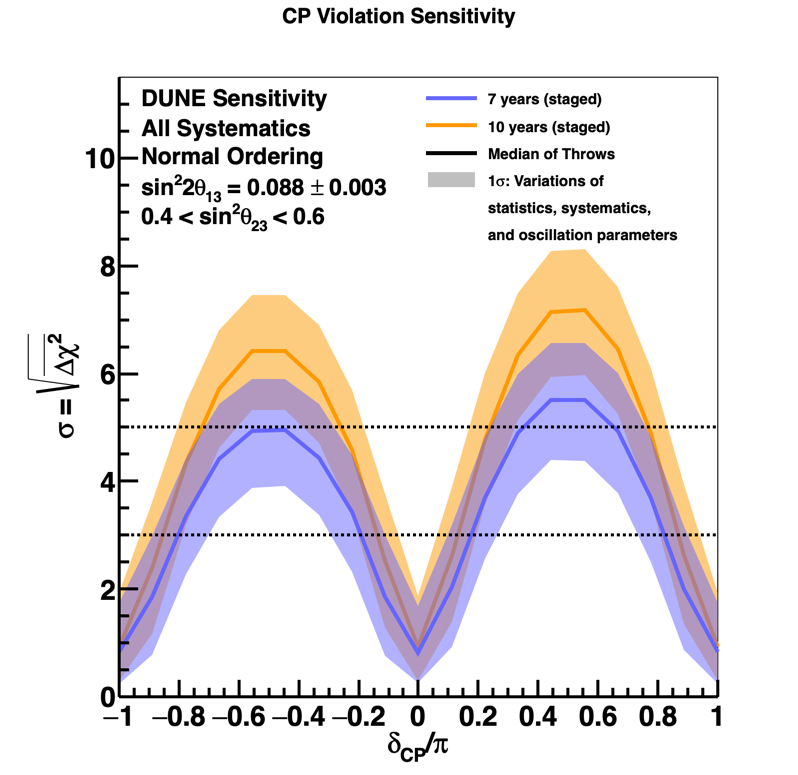
\includegraphics[width=0.95\linewidth]{cpv_two_exps_throws_nh_2019_v4.png}
	\caption[Significance of the DUNE determination of CP-violation as a function of \deltacp]{Significance of the DUNE determination of CP-violation (i.e.: \deltacp $\neq 0$ or $\pi$) as a function of the true value of \deltacp, for seven (blue) and ten (orange) years of exposure. True normal ordering is assumed. The width of the transparent bands cover 68\% of fits in which random throws are used to simulate statistical variations and select true values of the oscillation and systematic uncertainty parameters, constrained by pre-fit uncertainties. The solid lines show the median sensitivity.}
    \label{fig:cpv_nominal}
\end{figure}

Figure~\ref{fig:cpv_staging} shows the significance
with which CP violation can be determined for 75\% and 50\% of \deltacp values, and when $\deltacp=-\pi/2$, as a function of exposure in years, using the staging scenario described in Section~\ref{sec:physics-lbnosc-osc}. It is not possible for any experiment to provide 100\% coverage in \deltacp for a \dword{cpv} measurement because \dword{cpv} effects vanish at certain values of \deltacp. The changes in trajectory of the curves in the first three years results from the staging of far detector module installation; the change at 6 years is due to the upgrade from 1.2- to 2.4-MW beam power. The width of the bands show the impact of applying an external constraint on \sinstt{13}. As seen in Table~\ref{tab:milestones}, CP violation can be observed with 5$\sigma$ significance after about 7 years if \deltacp = $-\pi/2$ and after about 10 years for 50\% of \deltacp values. CP violation can be observed with 3$\sigma$ significance for 75\% of \deltacp values after about 13 years of running. Figure~\ref{fig:cpv_exposure} shows the same CP violation sensitivity as a function of exposure in kt-MW-years. In the left plot, the width of the bands shows the impact of applying an external constraint on \sinstt{13}, while in the right plot, the width of the bands is the result of varying the true value of \sinst{23} within the \dword{nufit} 90\% C.L. allowed region.

\begin{figure}[h!]
    \centering
		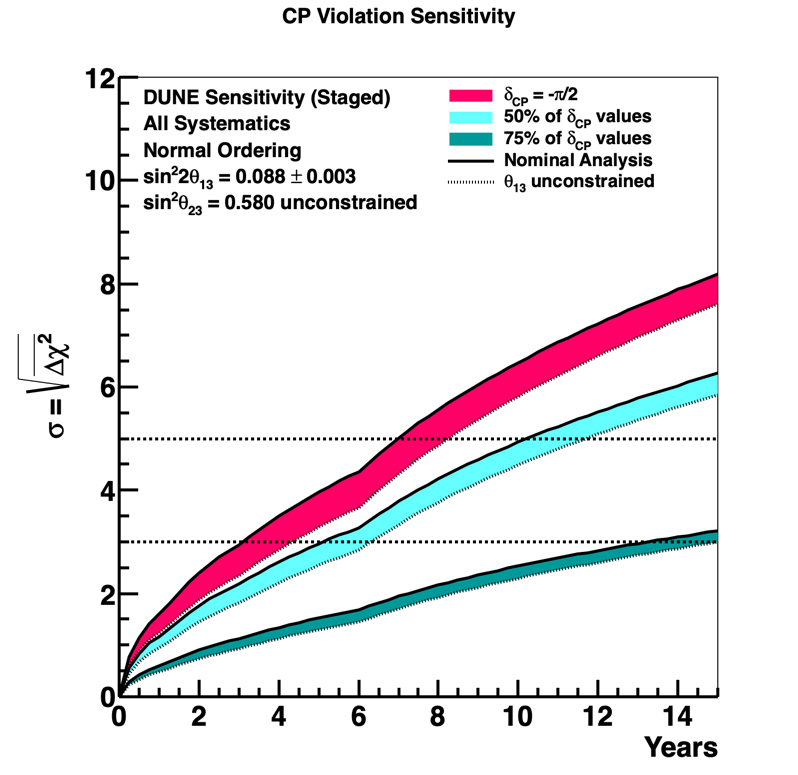
\includegraphics[width=0.95\linewidth]{cpv_exp_staging_varyconstr_nh_2019_v4.png}
	\caption[Significance of the DUNE determination of CP-violation as a function of time]{Significance of the DUNE determination of CP-violation (i.e.: \deltacp $\neq 0$ or $\pi$) for the case when \deltacp=$-\pi/2$, and for 50\% and 75\% of possible true \deltacp values, as a function of time in calendar years. True normal ordering is assumed. The width of the band shows the impact of applying an external constraint on \sinstt{13}.}
    \label{fig:cpv_staging}
\end{figure}

\begin{figure}[h!]
    \centering
    \begin{tabular}{cc}
		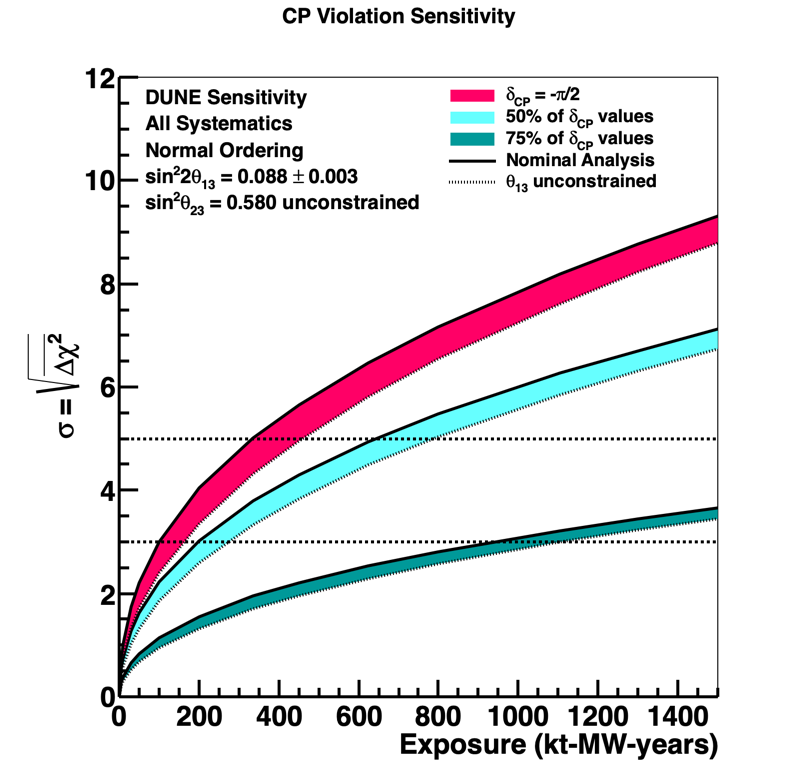
\includegraphics[width=0.475\linewidth]{cpv_exp_varyconstr_nh_2019_v4.png} &
		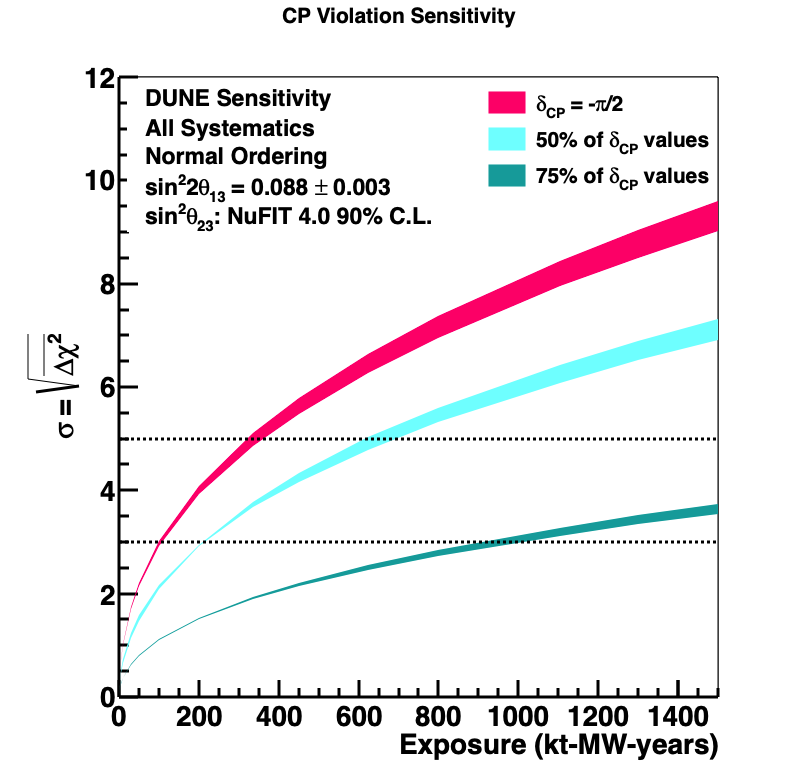
\includegraphics[width=0.475\linewidth]{cpv_exp_varyth23_nh_2019_v4.png}
    \end{tabular}
	\caption[Significance of the DUNE determination of CP-violation as a function of exposure]{Significance of the DUNE determination of CP-violation (i.e.: \deltacp $\neq 0$ or $\pi$) for the case when \deltacp=$-\pi/2$, and for 50\% and 75\% of possible true \deltacp values, as a function of exposure in kt-MW-years. True normal ordering is assumed. Left: The width of the band shows the impact of applying an external constraint on \sinstt{13}. Right: The width of the band shows the impact of varying the true value of \sinst{23} within the \dword{nufit} 90\% C.L. region.
% JU 1/24
For reference, 30, 100, 200, 336, 624, and \SI{1104}{\ktMWyr} correspond to 1.2, 3.1, 5.2, 7, 10, and 15 staged years, respectively.
% end JU 1/24
}
    \label{fig:cpv_exposure}
\end{figure}

\subsection{Mass Hierarchy}
\label{sec:physics-lbnosc-mh}


Figure~\ref{fig:mh_nominal} shows the significance with which the neutrino mass ordering can be determined as a function of the true value of \deltacp, using the same exposures and staging assumptions described in the previous section. The characteristic shape results from near degeneracy between matter and CP-violating effects that occurs near $\deltacp=\pi/2$ for true normal ordering.
As in the CP violation sensitivity, the solid curve represents the median sensitivity, the width of the transparent band represents 68\% of fits when random throws are used to simulate statistical variations and select true values of the oscillation and systematic uncertainty parameters, constrained by pre-fit uncertainties, and variation in the true value of \sinst{23} is responsible for a significant portion of this variation.

\begin{figure}[h!]
    \centering
		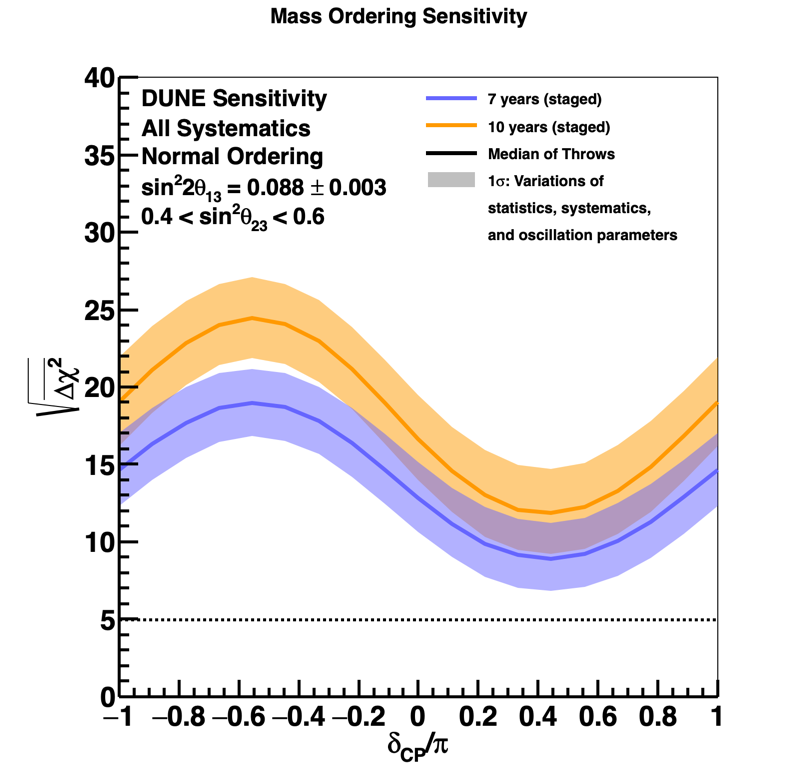
\includegraphics[width=0.95\linewidth]{mh_two_exps_throws_nh_2019_v4.png}
	\caption[Significance of the DUNE neutrino mass ordering determination, as a function of \deltacp]{Significance of the DUNE determination of the neutrino mass ordering, as a function of the true value of \deltacp, for seven (blue) and ten (orange) years of exposure. True normal ordering is assumed. The width of the transparent bands cover 68\% of fits in which random throws are used to simulate statistical variations and select true values of the oscillation and systematic uncertainty parameters, constrained by pre-fit uncertainties. The solid lines show the median sensitivity. }
    \label{fig:mh_nominal}
\end{figure}

Figure~\ref{fig:mh_staging} shows the significance
with which the neutrino mass ordering can be determined for 100\% of \deltacp values, and when $\deltacp=-\pi/2$, as a function of exposure in years. The width of the bands show the impact of applying an external constraint on \sinstt{13}. Figure~\ref{fig:mh_exposure} shows the same sensitivity as a function of exposure in kt-MW-years. As DUNE will be able to establish the neutrino mass ordering at the 5-$\sigma$ level for 100\% of \deltacp values after between two and three years, these plots extend only to seven years and 500 kt-MW-years, respectively.

\begin{figure}[h!]
    \centering
	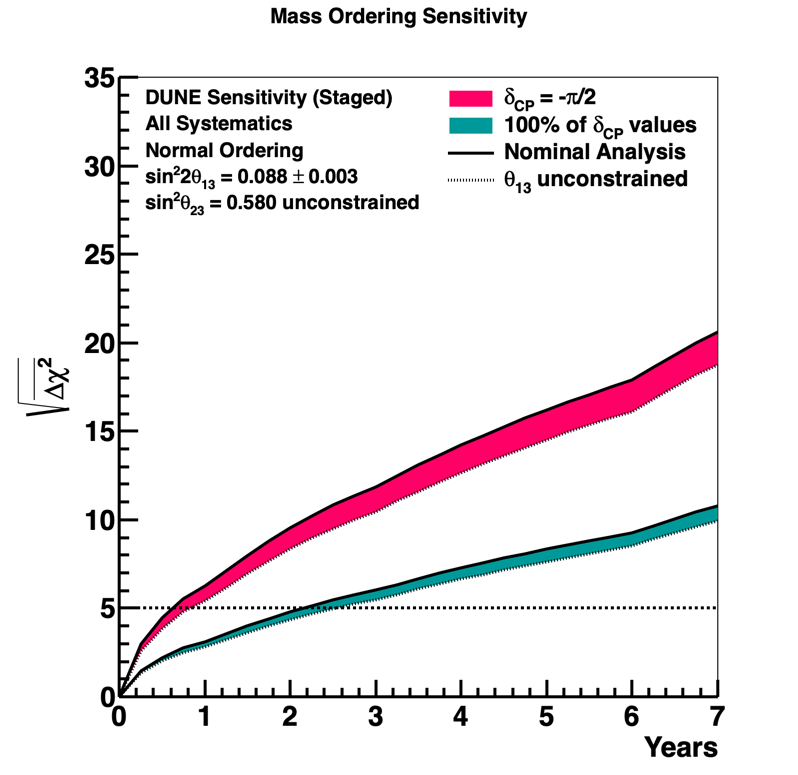
\includegraphics[width=0.95\linewidth]{mh_exp_staging_varyconstr_nh_2019_v4.png}	
	\caption[Significance of the DUNE neutrino mass ordering determination, as a function of time]{Significance of the DUNE determination of the neutrino mass ordering for the case when \deltacp=$-\pi/2$, and for 100\% of possible true \deltacp values, as a function of time in calendar years. True normal ordering is assumed. The width of the band shows the impact of applying an external constraint on \sinstt{13}.}
    \label{fig:mh_staging}
\end{figure}

\begin{figure}[h!]
    \centering
    \begin{tabular}{cc}
    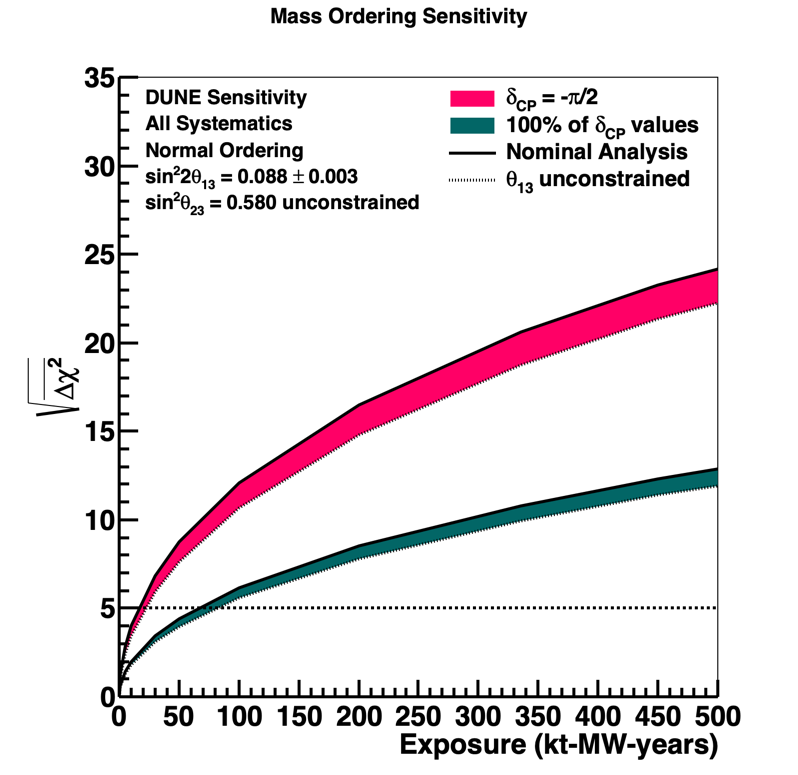
\includegraphics[width=0.475\linewidth]{mh_exp_varyconstr_nh_2019_v4.png} &
	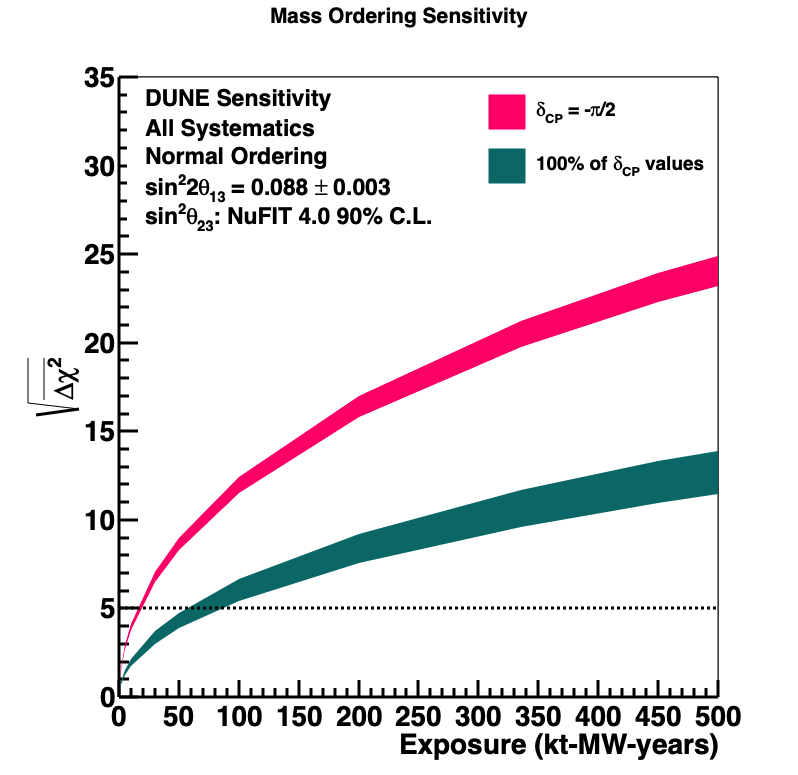
\includegraphics[width=0.475\linewidth]{mh_exp_varyth23_nh_2019_v4.png} 
	\end{tabular}
	\caption[Significance of the DUNE neutrino mass ordering determination as a function of exposure]{Significance of the DUNE determination of the neutrino mass ordering for the case when \deltacp=$-\pi/2$, and for 100\% of possible true \deltacp values, as a function of exposure in kt-MW-years. True normal ordering is assumed. Left: The width of the band shows the impact of applying an external constraint on \sinstt{13}. Right: The width of the band shows the impact of varying the true value of \sinst{23} within the \dword{nufit} 90\% C.L. region.
% JU 1/24
For reference, 30, 100, 200, and \SI{336}{\ktMWyr} correspond to 1.2, 3.1, 5.2, and 7  staged years, respectively.
% end JU 1/24
}
    \label{fig:mh_exposure}
\end{figure}

Studies have indicated that special attention must be paid to the statistical interpretation of neutrino mass ordering sensitivities~\cite{Qian:2012zn,Blennow:2013oma} because the $\Delta\chi^2$ metric does not follow the expected chi-squared function for one degree of freedom, so the interpretation of the sensitivity given by the Asimov data set is less straightforward. The error band on the mass ordering sensitivity shown in Figure~\ref{fig:mh_nominal} includes this effect using the technique of statistical throws described in Section~\ref{sect:methods-dunefits}. The effect of statistical fluctuation and systematic uncertainties in the neutrino mass ordering sensitivity for values of \sinst{23} in the range 0.56 to 0.60 is explored using random throws to determine the 1- and 2-$\sigma$ ranges of possible sensitivity. The resulting range of sensitivities is shown in Figure~\ref{fig:mh_stats}, for 10 years of exposure.

\begin{figure}[h!]
    \centering
		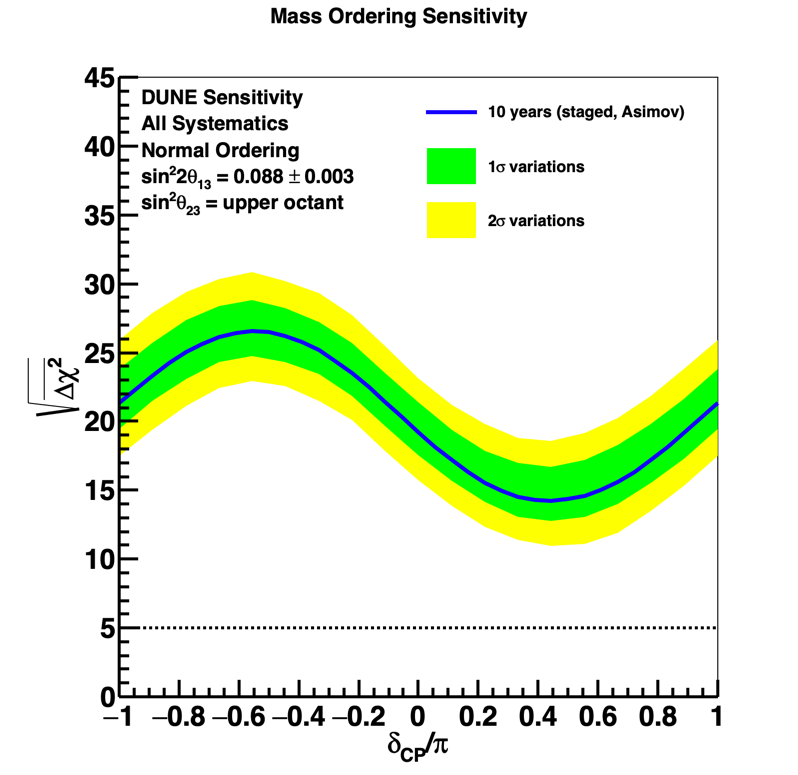
\includegraphics[width=0.95\linewidth]{mh_10yr_throws_nh_brazil_2019_v4.png}
	\caption[Significance of the DUNE determination of the neutrino mass ordering: statistical and systematic variations]{Significance of the DUNE determination of the neutrino mass ordering, as a function of the true value of \deltacp, for ten years of exposure. True normal ordering is assumed. The width of the bands are 1- and 2-$\sigma$ statistical and systematic variations. The blue curve shows sensitivity for the Asimov set.}
    \label{fig:mh_stats}
\end{figure}

\subsection{Precision Oscillation Parameter Measurements}
\label{sec:physics-lbnosc-prec}

In addition to the discovery potential for neutrino mass hierarchy and \dword{cpv}, 
\dword{dune} will improve the precision on key parameters that govern neutrino oscillations, including: \deltacp, $\sin^22\theta_{13}$, \dm{31}, $\sin^2\theta_{23}$ and the octant of $\theta_{23}$. 

Figure~\ref{fig:dcpresvdcp} shows the resolution, in degrees, of DUNE's measurement of \deltacp, as a function of the true value of \deltacp. The resolution of this measurement is significantly better near CP-conserving values of \deltacp, compared to maximally CP-violating values. For fifteen years of exposure, resolutions between five and fifteen degrees are possible, depending on the true value of \deltacp. A smoothing algorithm has been applied to interpolate between values of \deltacp at which the full analysis has been performed.

\begin{figure}[h!]
    \centering
		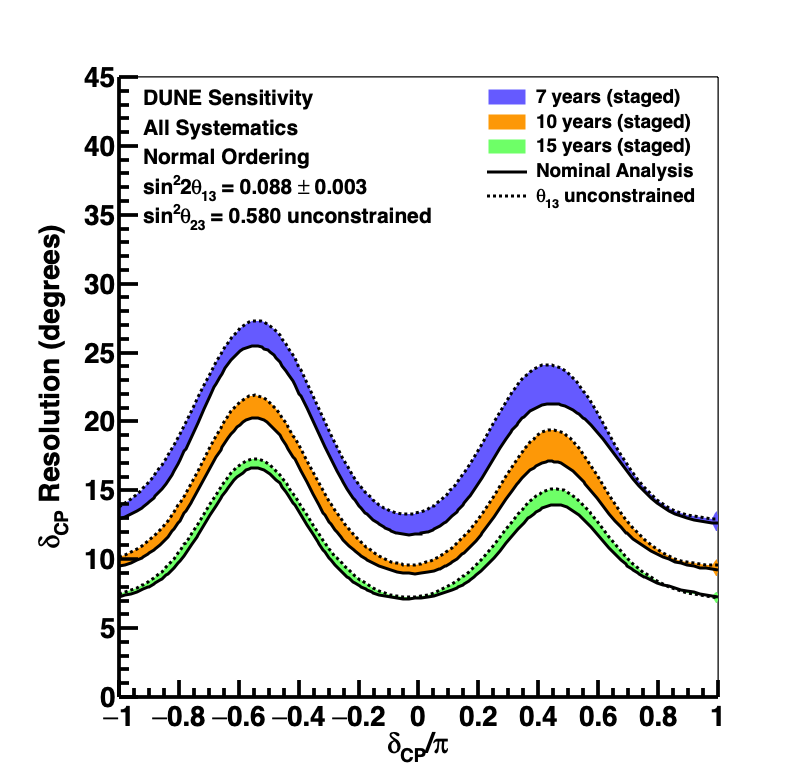
\includegraphics[width=0.95\linewidth]{dcpresvdcp_smooth_v4.png}
	\caption[Resolution for the DUNE measurement of \deltacp as a function of \deltacp]
	{Resolution in degrees for the DUNE measurement of \deltacp, as a function of the true value of \deltacp, for seven (blue), ten (orange), and fifteen (green) years of exposure. True normal ordering is assumed. The width of the band shows the impact of applying an external constraint on \sinstt{13}.}
    \label{fig:dcpresvdcp}
\end{figure}

Figures \ref{fig:appres_exp} and  \ref{fig:disres_exp} show the resolution of DUNE's measurements of \deltacp and \sinstt{13} and of \sinstt{23} and $\Delta m^{2}_{32}$, respectively, as a function of exposure in kt-MW-years. As seen in Figure~\ref{fig:dcpresvdcp}, the \deltacp resolution varies significantly with the true value of \deltacp, but for favorable values, resolutions near five degrees are possible for large exposure. The DUNE measurement of \sinstt{13} approaches the precision of reactor experiments for high exposure, allowing a comparison between the two results, which is of interest as a test of the unitarity of the PMNS matrix. 

\begin{figure}[h!]
    \centering
    \begin{tabular}{cc}
		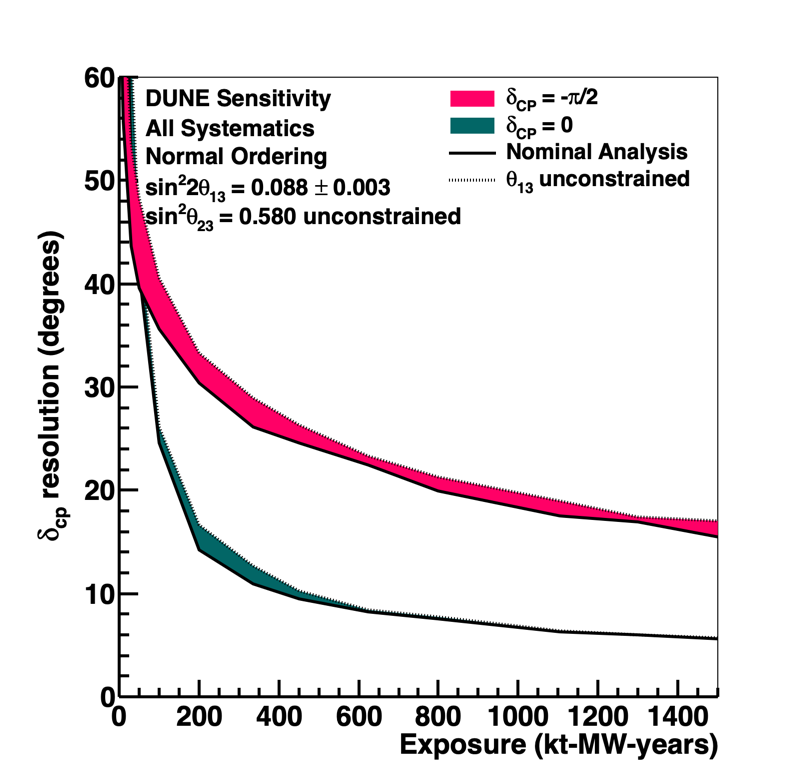
\includegraphics[width=0.475\linewidth]{dcpres_exp_varyconstr_nh_2019_v4.png} &
		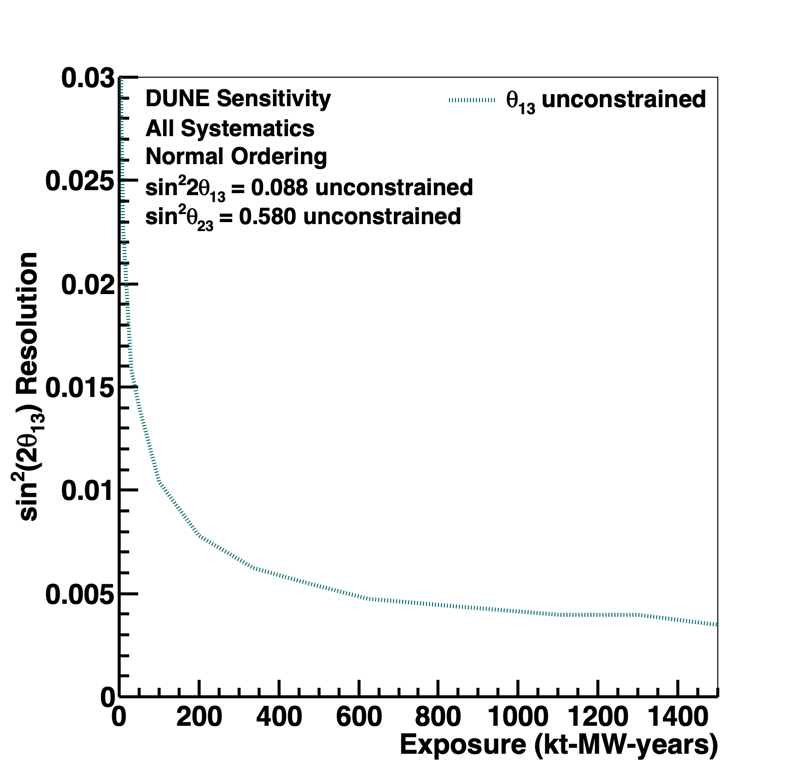
\includegraphics[width=0.475\linewidth]{th13res_exp_varyconstr_nh_2019_v4.png} 
	\end{tabular}  
	\caption[Resolution of DUNE measurements of \deltacp and \sinstt{13}, as a function of exposure]{Resolution of DUNE measurements of \deltacp (left) and \sinstt{13} (right), as a function of exposure in kt-MW-years. As seen in Figure~\ref{fig:dcpresvdcp}, the \deltacp resolution has a significant dependence on the true value of \deltacp, so curves for $\deltacp=-\pi/2$ (red) and $\deltacp=0$ (green) are shown. The width of the band shows the impact of applying an external constraint on \sinstt{13}. For the \sinstt{13} resolution, an external constraint does not make sense, so only the unconstrained curve is shown.
% JU 1/24
For reference, 30, 100, 200, 336, 624, and \SI{1104}{\ktMWyr} correspond to 1.2, 3.1, 5.2, 7, 10, and 15 staged years, respectively.
% end JU 1/24
}
    \label{fig:appres_exp}
\end{figure}

\begin{figure}[h!]
    \centering
    \begin{tabular}{cc}
		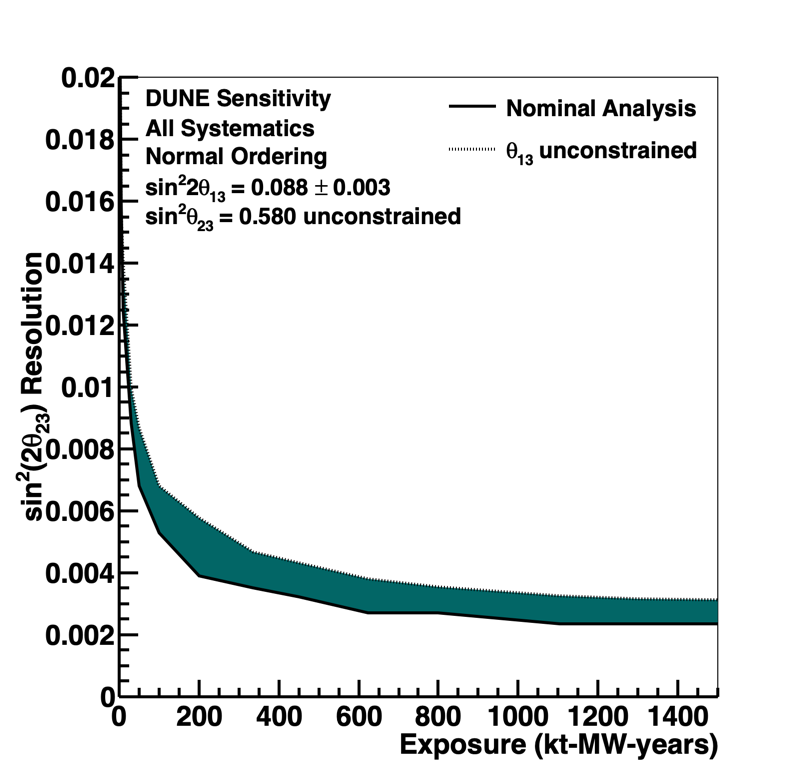
\includegraphics[width=0.475\linewidth]{th23res_exp_varyconstr_nh_2019_v4.png} &
		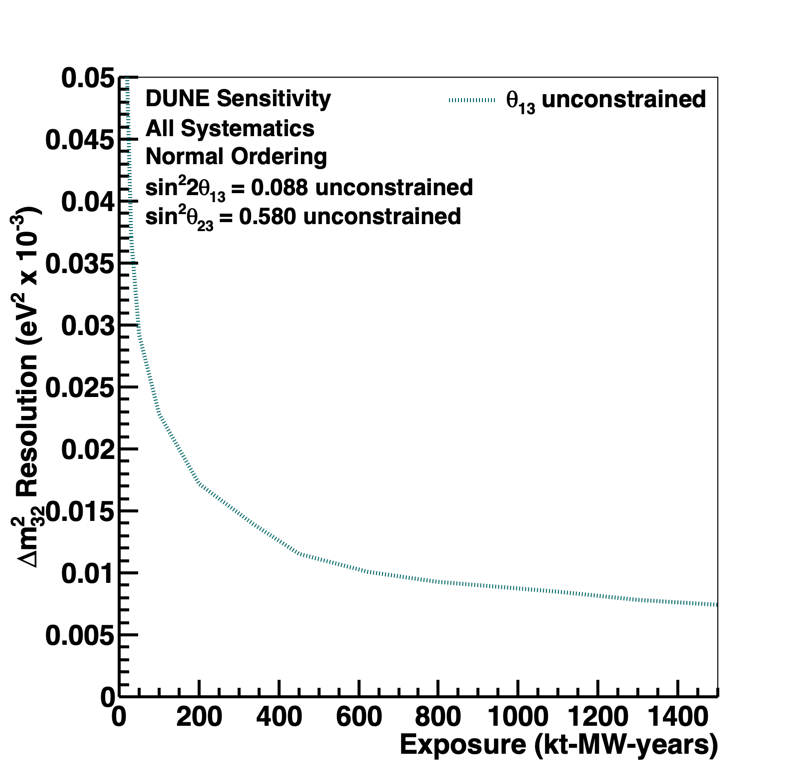
\includegraphics[width=0.475\linewidth]{dmsqres_exp_varyconstr_nh_2019_v4.png} 
	\end{tabular}  
	\caption[Resolution of DUNE measurements of \deltacp and \sinstt{13}, as a function of exposure]{Resolution of DUNE measurements of \sinstt{23} (left) and $\Delta m^{2}_{32}$ (right), as a function of exposure in kt-MW-years. The width of the band for the \sinstt{23} resolution shows the impact of applying an external constraint on \sinstt{13}. For the $\Delta m^{2}_{32}$ resolution, an external constraint does not have a significant impact, so only the unconstrained curve is shown.
% JU 1/24
For reference, 30, 100, 200, 336, 624, and \SI{1104}{\ktMWyr} correspond to 1.2, 3.1, 5.2, 7, 10, and 15 staged years, respectively.
% end JU 1/24
}
    \label{fig:disres_exp}
\end{figure}

One of the primary physics goals for DUNE is the simultaneous measurement of all oscillation parameters governing long-baseline neutrino oscillation, without a need for external constraints. Figure~\ref{fig:res_th13vdcp} shows the 90\% C.L. allowed regions for \sinstt{13} and \deltacp for 7, 10, and 15 years of running, when no external constraints are applied, compared to the current measurements from world data. Note that a degenerate lobe at higher values of \sinstt{13} is present in the 7-year exposure, but is resolved for higher exposures. Figure~\ref{fig:res_th23vdcp} shows the two-dimensional allowed regions for \sinst{23} and \deltacp. Figure~\ref{fig:res_th23vdcp_degen} explores the resolution sensitivity that is expected for values of \sinst{23} different from the \dword{nufit} central value. It is interesting to note that the lower exposure, opposite octant solutions for \sinst{23} are allowed at 90\% C.L. in the absence of an external constraint on \sinstt{13}; however, at the 10 year exposure, this degeneracy is resolved by DUNE data without external constraint.

\begin{figure}[h!]
    \centering
		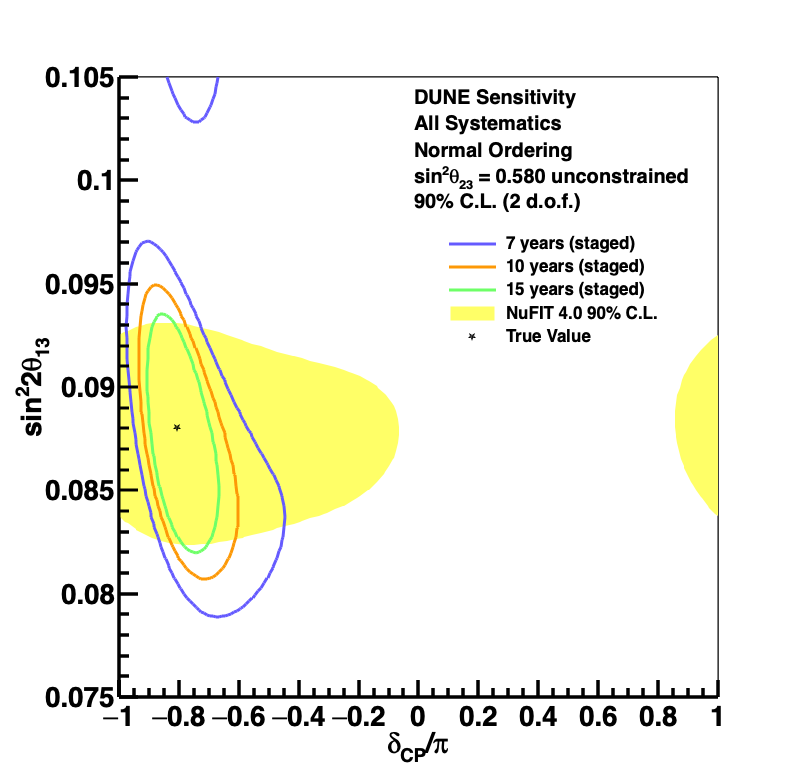
\includegraphics[width=0.95\linewidth]{graphics/bubbles_q13_2019_fulldisclosure.png}
	\caption[Two-dimensional 90\% C.L. region in \sinstt{13} and \deltacp]{Two-dimensional 90\% C.L. region in \sinstt{13} and \deltacp, for 7, 10, and 15 years of exposure, with equal running in neutrino and antineutrino mode. The 90\% C. L. region for the \dword{nufit} global fit is shown in yellow for comparison. The true values of the oscillation parameters are assumed to be the central values of the \dword{nufit} global fit and the oscillation parameters governing long-baseline oscillation are unconstrained.}
    \label{fig:res_th13vdcp}
\end{figure}

\begin{figure}[h!]
    \centering
		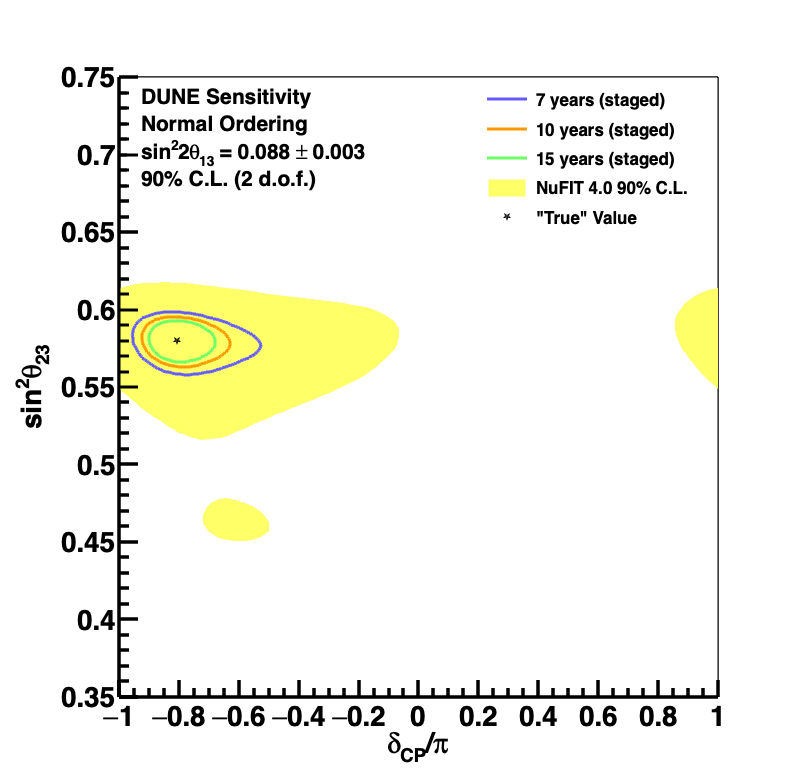
\includegraphics[width=0.95\linewidth]{bubbles_q23_asimov0_2019.png}
	\caption[Two-dimensional 90\% C.L. region in \sinst{23} and \deltacp]{Two-dimensional 90\% C.L. region in \sinst{23} and \deltacp, for 7, 10, and 15 years of exposure, with equal running in neutrino and antineutrino mode. The 90\% C. L. region for the \dword{nufit} global fit is shown in yellow for comparison. The true values of the oscillation parameters are assumed to be the central values of the \dword{nufit} global fit and \sinstt{13} is constrained by \dword{nufit}}
    \label{fig:res_th23vdcp}
\end{figure}

\begin{figure}[h!]
    \centering
    \begin{tabular}{cc}
		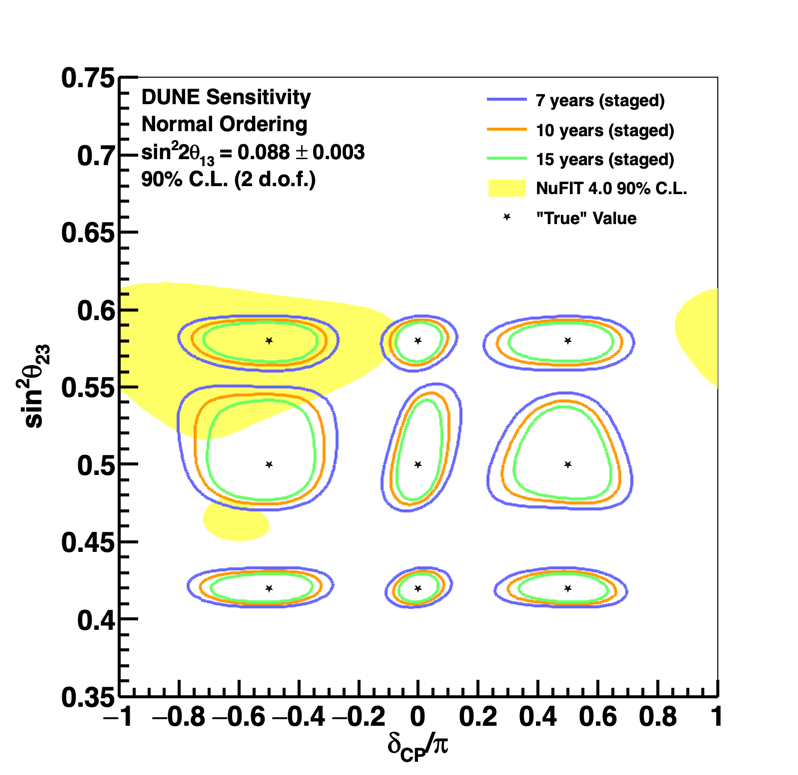
\includegraphics[width=0.475\linewidth]{bubbles_q23_2019_v4.png} &
		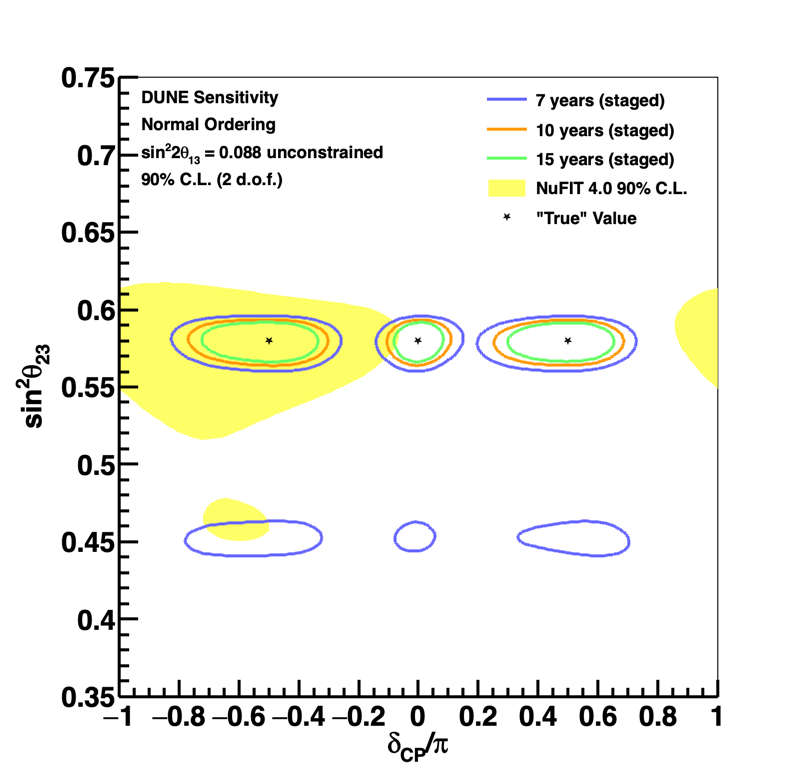
\includegraphics[width=0.475\linewidth]{bubbles_q23_nopen_2019_v4.png} 
	\end{tabular}  
	\caption[Two-dimensional 90\% C.L. region in \sinst{23} and \deltacp]{Two-dimensional 90\% C.L. region in \sinst{23} and \deltacp, for 7, 10, and 15 years of exposure, with equal running in neutrino and antineutrino mode. The 90\% C.L. region for the \dword{nufit} global fit is shown in yellow for comparison. Several possible true values of the oscillation parameters, denoted by stars, are considered, and \sinstt{13} is constrained (left) or unconstrained (right) by \dword{nufit}. In the plot on the right, only one value for \sinst{23} is shown; without the constraint on \sinstt{13}, degenerate regions are allowed for lower exposures.}
    \label{fig:res_th23vdcp_degen}
\end{figure}

The measurement of $\nu_\mu \rightarrow \nu_\mu$ oscillations is sensitive to $\sin ^2 2 \theta_{23}$, whereas the measurement of $\nu_\mu \rightarrow \nu_e$ oscillations is sensitive to $\sin^2 \theta_{23}$.  A combination of both $\nu_e$ appearance and $\nu_\mu$ disappearance measurements can probe both maximal mixing and
the $\theta_{23}$ octant.  
Figure~\ref{fig:lbloctant} shows the sensitivity to determining the octant as a function of the true value of $\sinst{23}$.

\begin{figure}[h!]
    \centering
		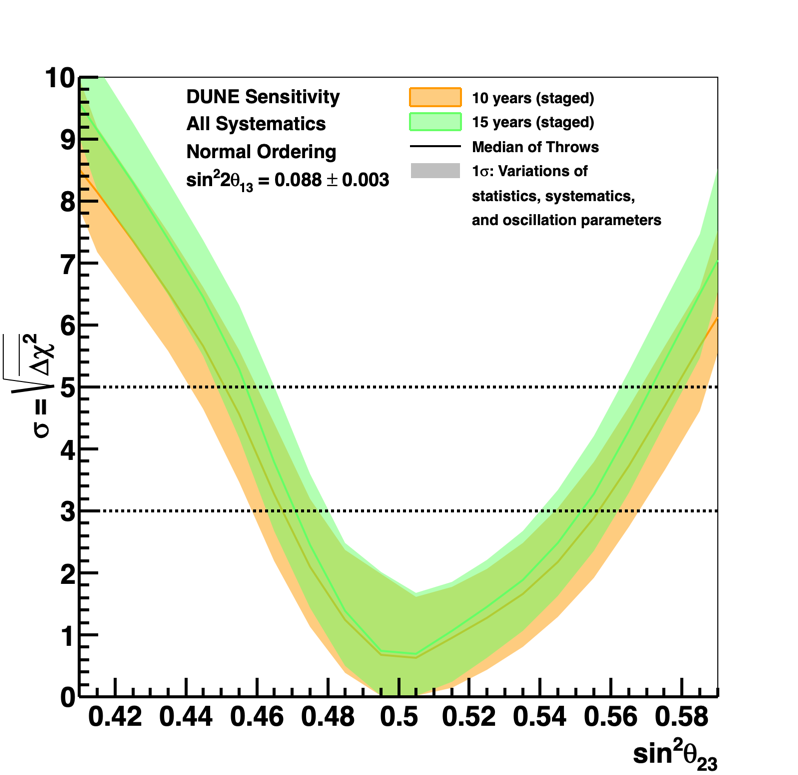
\includegraphics[width=0.75\linewidth]{octant_no_2019_v4.png}
	\caption[Sensitivity of determination of the $\theta_{23}$ octant as a function of \sinst{23}]{Sensitivity to determination of the $\theta_{23}$ octant as a function of the true value of \sinst{23}, for ten (orange) and fifteen (green) years of exposure. True normal ordering is assumed. The width of the transparent bands cover 68\% of fits in which random throws are used to simulate statistical variations and select true values of the oscillation and systematic uncertainty parameters, constrained by pre-fit uncertainties. The solid lines show the median sensitivity.}
    \label{fig:lbloctant}
\end{figure}

\subsection{Impact of Oscillation Parameter Central Values}
\label{sec:physics-lbnosc-oscvar}
The sensitivity results presented in the preceding sections assume that the true values of the parameters governing long-baseline neutrino oscillation are the central values of the \dword{nufit} global fit, given in Table~\ref{tab:oscpar_nufit}. In this section, variations in DUNE sensitivity with other possible true values of the oscillation parameters are explored.
Figures \ref{fig:th23var}, \ref{fig:th13var}, and \ref{fig:dmsqvar} show DUNE sensitivity to CP violation and neutrino mass ordering when the true values of $\theta_{23}$, $\theta_{13}$, and $\Delta m^{2}_{32}$, respectively, vary within the 3$\sigma$ range allowed by \dword{nufit}. The largest effect is the variation in sensitivity with the true value of $\theta_{23}$, where degeneracy with $\deltacp$ and matter effects are significant. Values of $\theta_{23}$ in the lower octant lead to the best sensitivity to CP violation and the worst sensitivity to neutrino mass ordering, while the reverse is true for the upper octant. DUNE sensitivity for the case of maximal mixing is also shown. The true values of $\theta_{13}$ and $\Delta m^2_{32}$ are highly constrained by global data and, within these constraints, do not have a dramatic impact on DUNE sensitivity.  

\begin{figure}[h!]
    \centering
    \begin{tabular}{cc}
		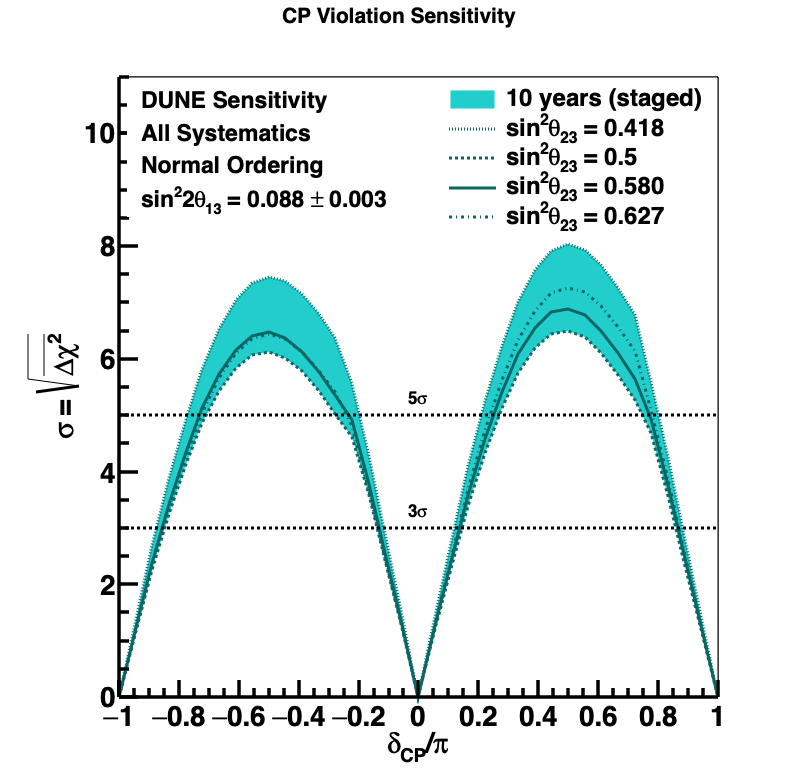
\includegraphics[width=0.475\linewidth]{cpv_varyth23_2019_v4.png} &
		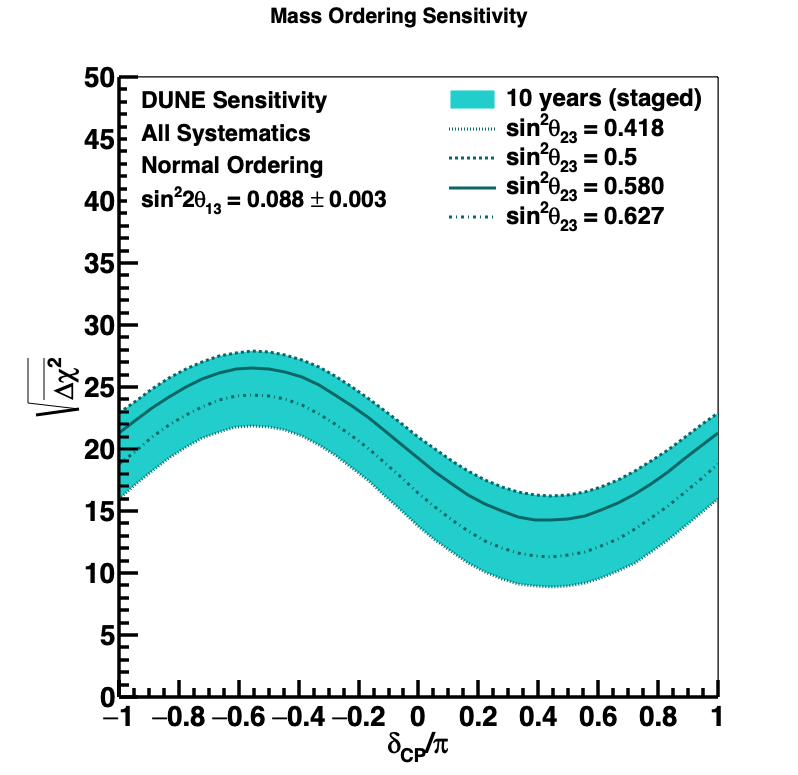
\includegraphics[width=0.475\linewidth]{mh_varyth23_2019_v4.png}
	\end{tabular}
	\caption[Sensitivity to CP violation and neutrino mass ordering, as a function of $\deltacp$]{Sensitivity to CP violation (left) and neutrino mass ordering (right), as a function of the true value of $\deltacp$, for 10 years of exposure, with equal running in neutrino and antineutrino mode. Curves are shown for true values of $\theta_{23}$ corresponding to the 3$\sigma$ range of values allowed by \dword{nufit}, as well as the \dword{nufit} central value and maximal mixing. The nominal sensitivity analysis is performed.}
    \label{fig:th23var}
\end{figure}

\begin{figure}[h!]
    \centering
    \begin{tabular}{cc}
		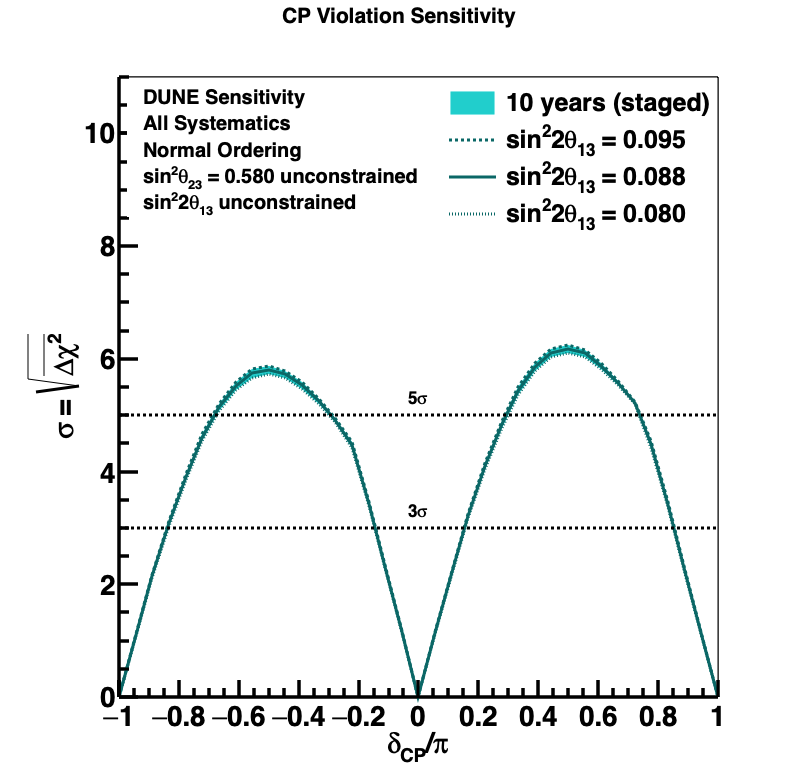
\includegraphics[width=0.475\linewidth]{cpv_varyth13_2019_v4.png} &
		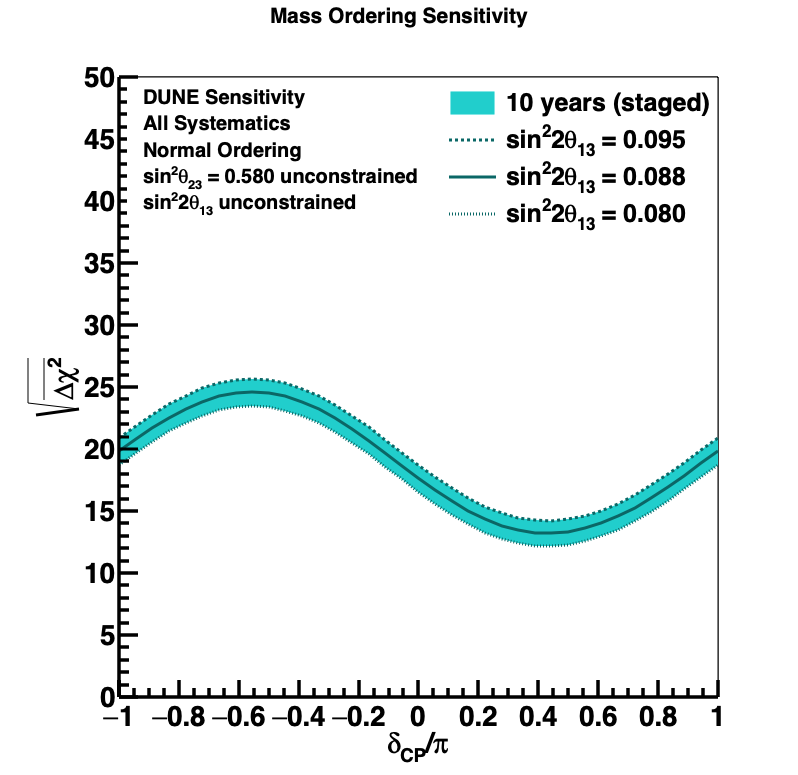
\includegraphics[width=0.475\linewidth]{mh_varyth13_2019_v4.png}
	\end{tabular}
	\caption[Sensitivity to CP violation and neutrino mass ordering, as a function of $\deltacp$]{Sensitivity to CP violation (left) and neutrino mass ordering (right), as a function of the true value of $\deltacp$, for 10 years of exposure, with equal running in neutrino and antineutrino mode. Curves are shown for true values of $\theta_{13}$ corresponding to the 3$\sigma$ range of values allowed by \dword{nufit}, as well as the \dword{nufit} central value. The nominal sensitivity analysis is performed, with the exception that $\theta_{13}$ is not constrained at the NuFit4.0 central value in the fit.}
    \label{fig:th13var}
\end{figure}

\begin{figure}[h!]
    \centering
    \begin{tabular}{cc}
		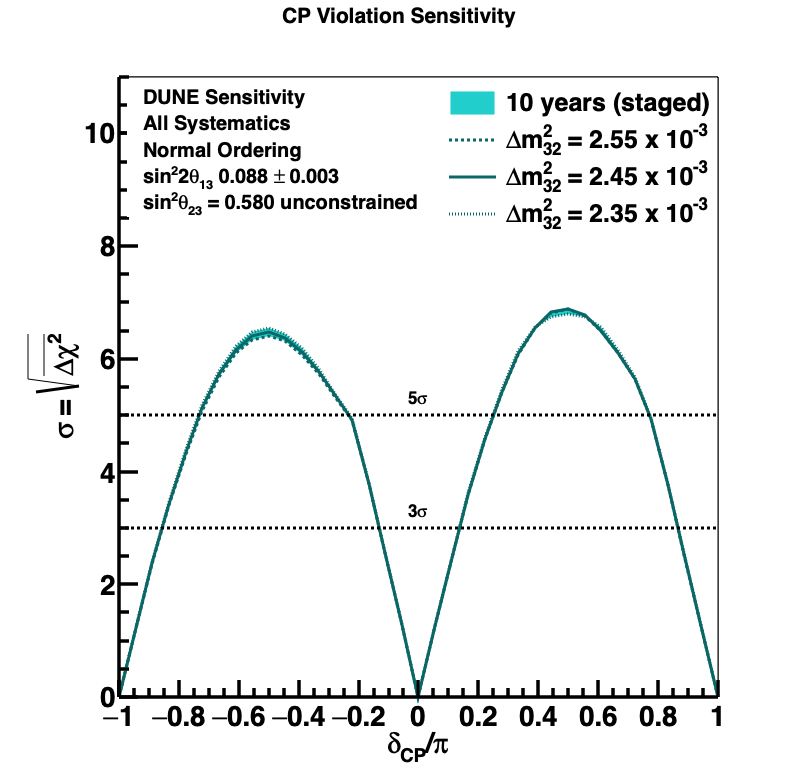
\includegraphics[width=0.475\linewidth]{cpv_varydmsq_2019_v4.png} &
		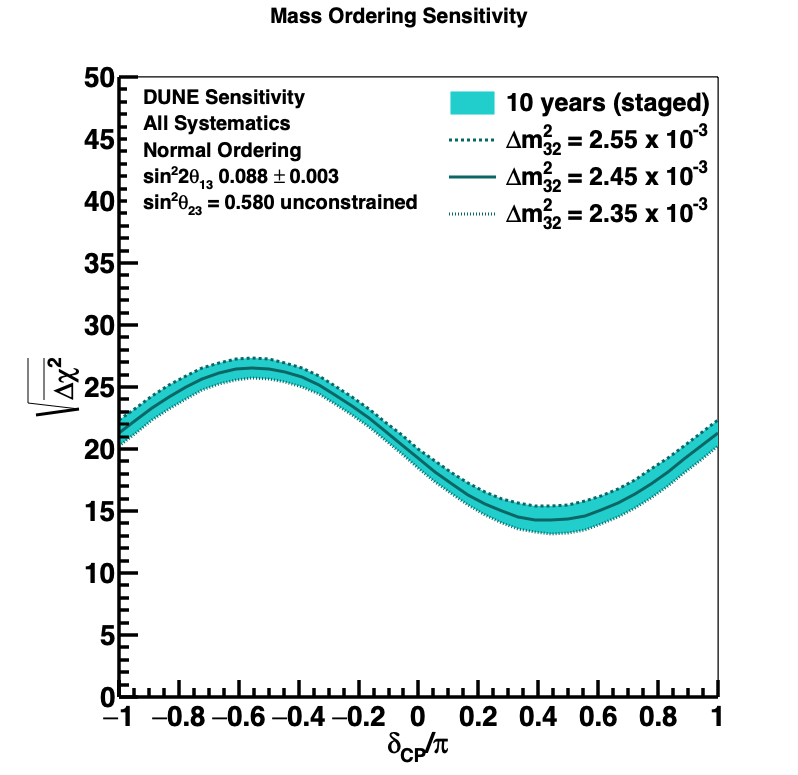
\includegraphics[width=0.475\linewidth]{mh_varydmsq_2019_v4.png}
	\end{tabular}
	\caption[Sensitivity to CP violation and neutrino mass ordering, as a function of $\deltacp$]{Sensitivity to CP violation (left) and neutrino mass ordering (right), as a function of the true value of $\deltacp$, for 10 years of exposure, with equal running in neutrino and antineutrino mode. Curves are shown for true values of $\Delta m^2_{32}$ corresponding to the 3$\sigma$ range of values allowed by \dword{nufit}, as well as the \dword{nufit} central value. The nominal sensitivity analysis is performed.}
    \label{fig:dmsqvar}
\end{figure}

\subsection{Impact of Systematic Uncertainties}
\label{sec:physics-lbnosc-systresults}

Implementation of systematic uncertainties in the nominal fits are described in Sections~\ref{sec:nu-osc-04}, \ref{sec:nu-osc-05}, and \ref{sec:physics-lbnosc-syst}. All considered systematic parameters are summarized in Table~\ref{tab:systcheatsheet}. %Figure~\ref{fig:results_systs} shows the impact of these systematic uncertainties on the sensitivity to CP violation, neutrino mass ordering, and \deltacp resolution, relative to the case where no systematic uncertainties are considered. 
In the nominal fits, many systematic uncertainties are constrained by DUNE data, as described in the following section.

\begin{longtable}{ll}\hline \hline
Brief Name & Description of Uncertainty \\  \hline \hline
\textbf{Flux:} & \\
flux[N] & Nth component of flux PCA \\ \hline
\textbf{Interaction Model:} & \\
MaCCQE & Axial mass for CCQE \\
VecFFCCQEshape & Choice of CCQE vector form factors \\
MaCCRES & Axial mass for CC resonance \\
MvCCRES & Vector mass for CC resonance \\
Theta Delta2Npi & $\theta_{\pi}$ distribution in decaying $\Delta$ rest frame \\
AhtBY & $A_{HT}$ higher-twist param in BY model scaling variable $\epsilon_{\omega}$ \\
BhtBY & $B_{HT}$ higher-twist param in BY model scaling variable $\epsilon_{\omega}$ \\
CV1uBY & $C_{V1u}$ valence GRV98 PDF correction param in BY model \\
CV2uBY & $C_{V2u}$ valence GRV98 PDF correction param in BY model \\
MaNCEL & Axial mass for NC elastic \\
MaNCRES & Axial mass for NC resonance \\
MvNCRES & Vector mass for NC resonance \\
FrCEx N & Nucleon charge exchange probability \\
FrElas N & Nucleon elastic reaction probability \\
FrInel N & Nucleon inelastic reaction probability \\
FrAbs N & Nucleon absorption probability \\
FrPiProd N & Nucleon $\pi$-production probability \\
FrCEx pi & $\pi$ charge exchange probability \\
FrElas pi & $\pi$ elastic reaction probability \\
FrInel pi & $\pi$ inelastic reaction probability \\
FrAbs pi & $\pi$ absorption probability \\
FrPiProd pi & $\pi$ $\pi$-production probability \\
BeRPA A & Random Phase Approximation tune: controls low $Q^{2}$ \\
BeRPA B &  Random Phase Approximation tune: controls low-mid $Q^{2}$\\
BeRPA D & Random Phase Approximation tune: controls mid $Q^{2}$ \\
Mnv2p2hGaussEnhancement & Extra strength into 2p2h \\
C12ToAr40 2p2hScaling nu & neutrino 2p2h Ar/C scaling \\
C12ToAr40 2p2hScaling nubar & antineutrino 2p2h Ar/C scaling \\
E2p2h [A,B] [nu,nubar] & 2p2h energy dependence \\
SPPLowQ2Suppression & Low $Q^{2}$ (empirical) suppression \\
MKSPP ReWeight & MK model - alternative strength in W \\
NR nu np CC 1Pi & Norm for $\nu + n/p \rightarrow l + 1\pi$ \\
NR [nu,nubar] [p,n] [CC,NC] [1,2,3]Pi & non-resonant pion production topology norms \\
nuenumu xsec ratio & \nue/\numu uncertainty in \nue unique phase space \\
nuenuebar xsec ratio & Modification of \nue/\numu and \anue/\anumu xsec \\ \hline
\textbf{Detector Effects:} & \\
FVNueFD & FD \nue fiducial volume \\
FVNueFD & FD \numu fiducial volume \\
FDRecoNueSyst & FD \nue selection \\
FDRecoNumuSyst & FD \numu selection \\
ChargedHadResFD & FD charged hadron resolution \\
EMResFD & FD electromagnetic shower resolution \\
MuonResFD & FD muon resolution \\
EMUncorrFD & FD electromagnetic shower energy scale \\
EScaleNFD & FD neutron visible energy scale \\
EScaleMuLArFD & FD muon energy scale \\
EScaleFD & FD overall energy scale \\
\hline
\hline
\caption[Definition of systematic uncertainty parameters]{Definition of systematic uncertainty parameters. The brief names are used in Figures \ref{fig:postfit_unc_ndfd} and \ref{fig:postfit_unc_vsexp}.} \\
\label{tab:systcheatsheet}
\end{longtable}


%\begin{figure}[h!]
%    \centering
%    \begin{tabular}{ccc}
%		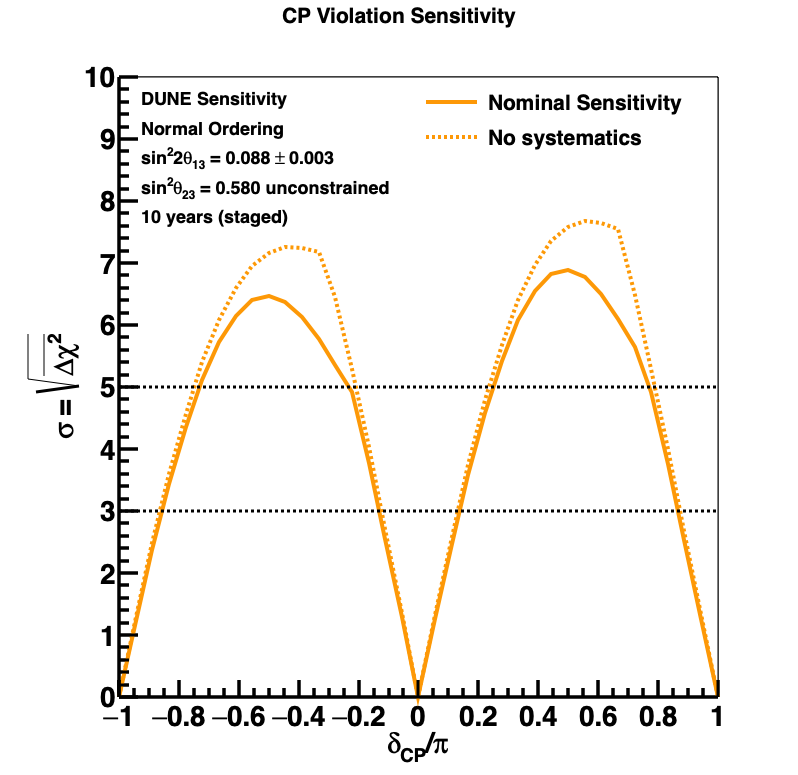
\includegraphics[width=0.3\linewidth]{cpv_nosyst_2019_v4.png} &
%		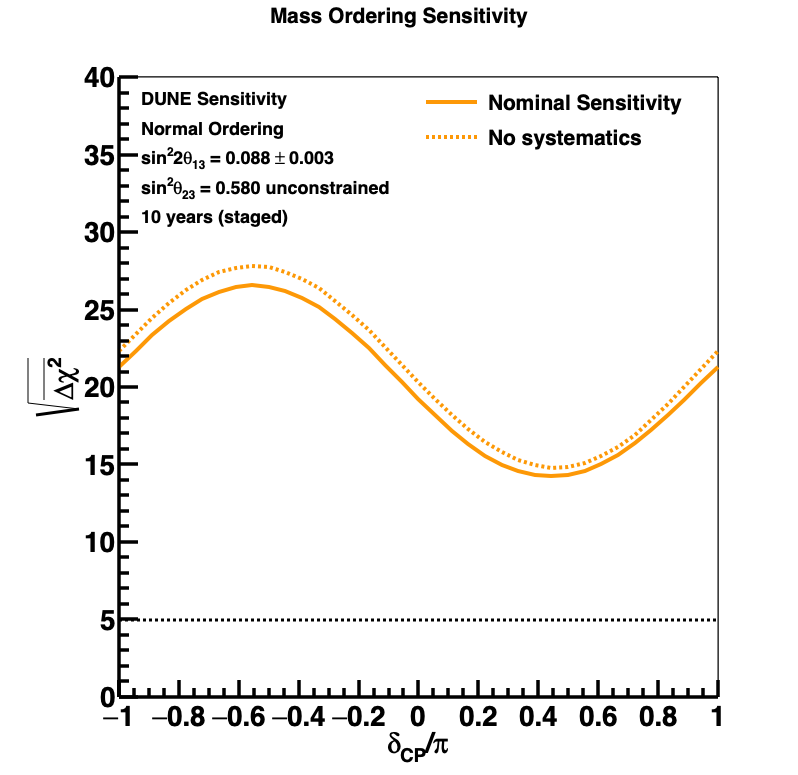
\includegraphics[width=0.3\linewidth]{mh_nosyst_2019_v4.png} &
%		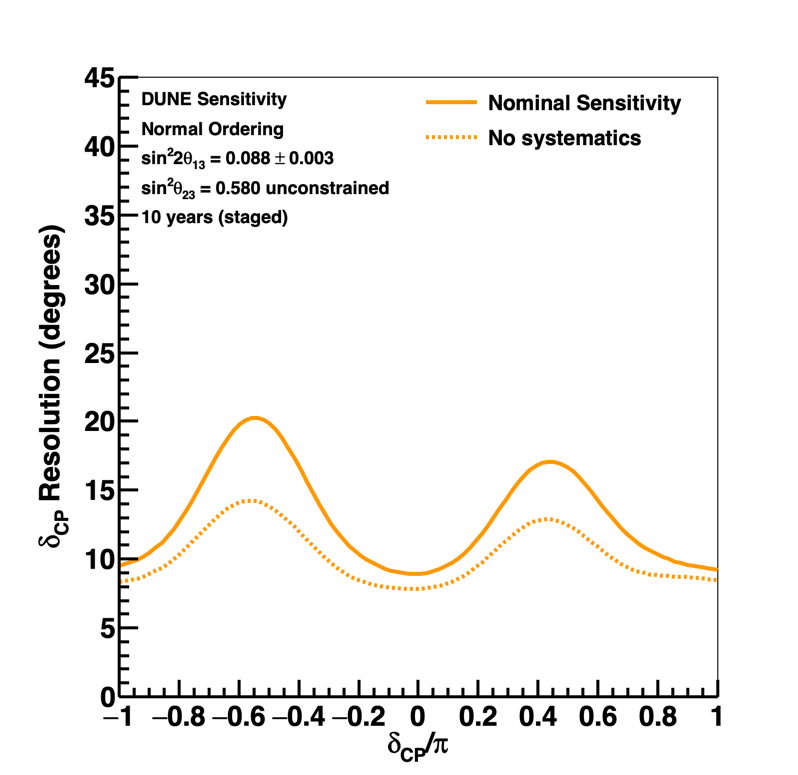
\includegraphics[width=0.3\linewidth]{dcpres_nosyst_2019_v4.png}
%	\end{tabular}
%	\caption[Sensitivity to CP violation, neutrino mass ordering, and \deltacp, as a function of  $\deltacp$]{Sensitivity to CP violation (left), neutrino mass ordering (middle), and \deltacp (right) as a function of the true value of $\deltacp$, for 10 years of exposure, with equal running in neutrino and antineutrino mode. The nominal Asimov sensitivity, including constraints from the near detector, is shown in the solid curve. The dashed curve shows the same sensitivity in the absence of systematic uncertainty.}
%    \label{fig:results_systs}
%\end{figure}

\subsubsection{Systematic Uncertainty Constraints}

Prefit uncertainties on flux and cross section parameters are at the level of $\sim$10\%. These uncertainties become constrained in the fit, especially by the \dword{nd}. Figure~\ref{fig:postfit_unc_ndfd} shows the level of constraint on each systematic parameter after the fit. The larger band shows the constraint that arises from the far detector alone, while the inner band shows the (much stronger) constraint from the near detector. Figure~\ref{fig:postfit_unc_vsexp} compares the parameter constraints for two different exposures. The wider band shows the \dword{nd}+\dword{fd} constraint expected after 7 years, and the narrower band shows the constraint after 15 years. The effect of increasing the exposure is very small because the \dword{nd} is already systematically limited in the \numu \dword{cc} channel after 7 years. The impact of adding the near detector is significant; flux and cross section parameters are very weakly constrained by the far detector alone. Parameters are implemented in such a way that there are no prefit correlations, but the constraints from the near detector cause parameters to become correlated, which is not shown in the figure.

Some uncertainties are not reduced by the \dword{nd}. For example, the energy scale parameters are treated as uncorrelated between detectors, so naturally the \dword{nd} does not constrain them. Several important cross section uncertainties are not constrained by the near detector. In particular, an uncertainty on the ratio of \numu to \nue cross sections is totally unconstrained. The most significant flux terms are constrained at the level of ~20\% of their \textit{a priori} values.  Less significant principal components have little impact on the observed distributions at either detector, and receive weaker constraints. Most cross section parameters that affect \dword{cc} interactions are well constrained.

\begin{dunefigure}[Post-fit systematic uncertainties]{fig:postfit_unc_ndfd}
{The ratio of post-fit to pre-fit uncertainties for various systematic parameters for a 15-year staged exposure. The red band shows the constraint from the \dword{fd} only in 15 years, while the green shows the \dword{nd}+\dword{fd} constraints. Systematic parameter names are defined in Table \ref{tab:systcheatsheet}.}
  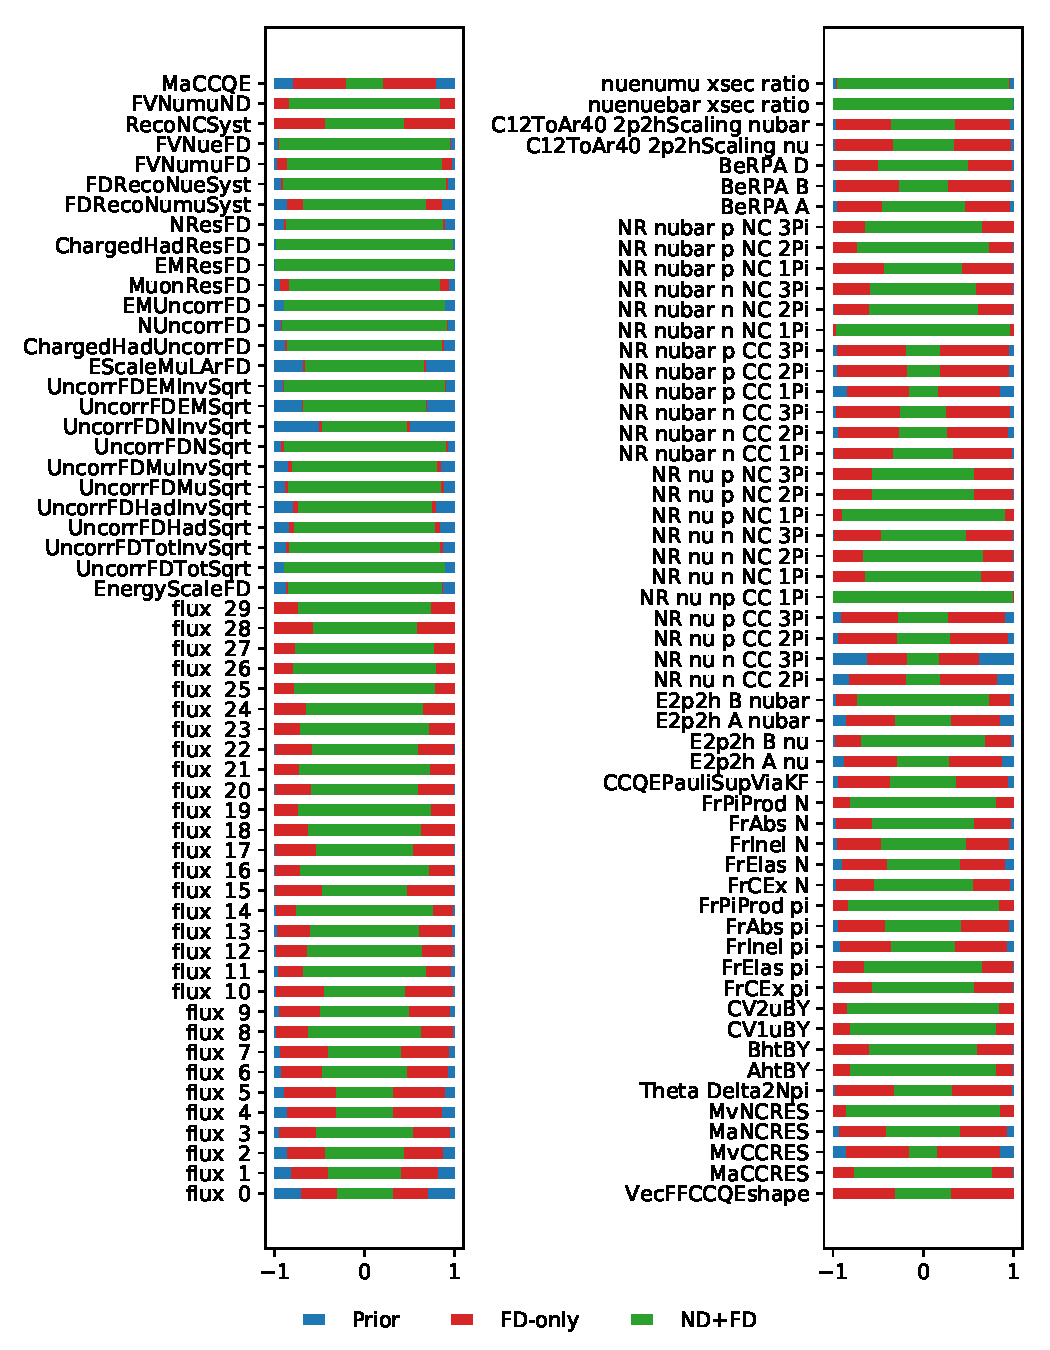
\includegraphics[width=0.8\textwidth]{nuisancePostFits_15_FDvsNDFD_th13_v4_1.pdf}
\end{dunefigure}

\begin{dunefigure}[Post-fit systematic uncertainties]{fig:postfit_unc_vsexp}
{The ratio of post-fit to pre-fit uncertainties for various systematic parameters for a \dword{nd}+\dword{fd} constraint after 7 and 15 years. The difference in parameter constraints due to increasing the exposure is very small. Systematic parameter names are defined in Table \ref{tab:systcheatsheet}.}
  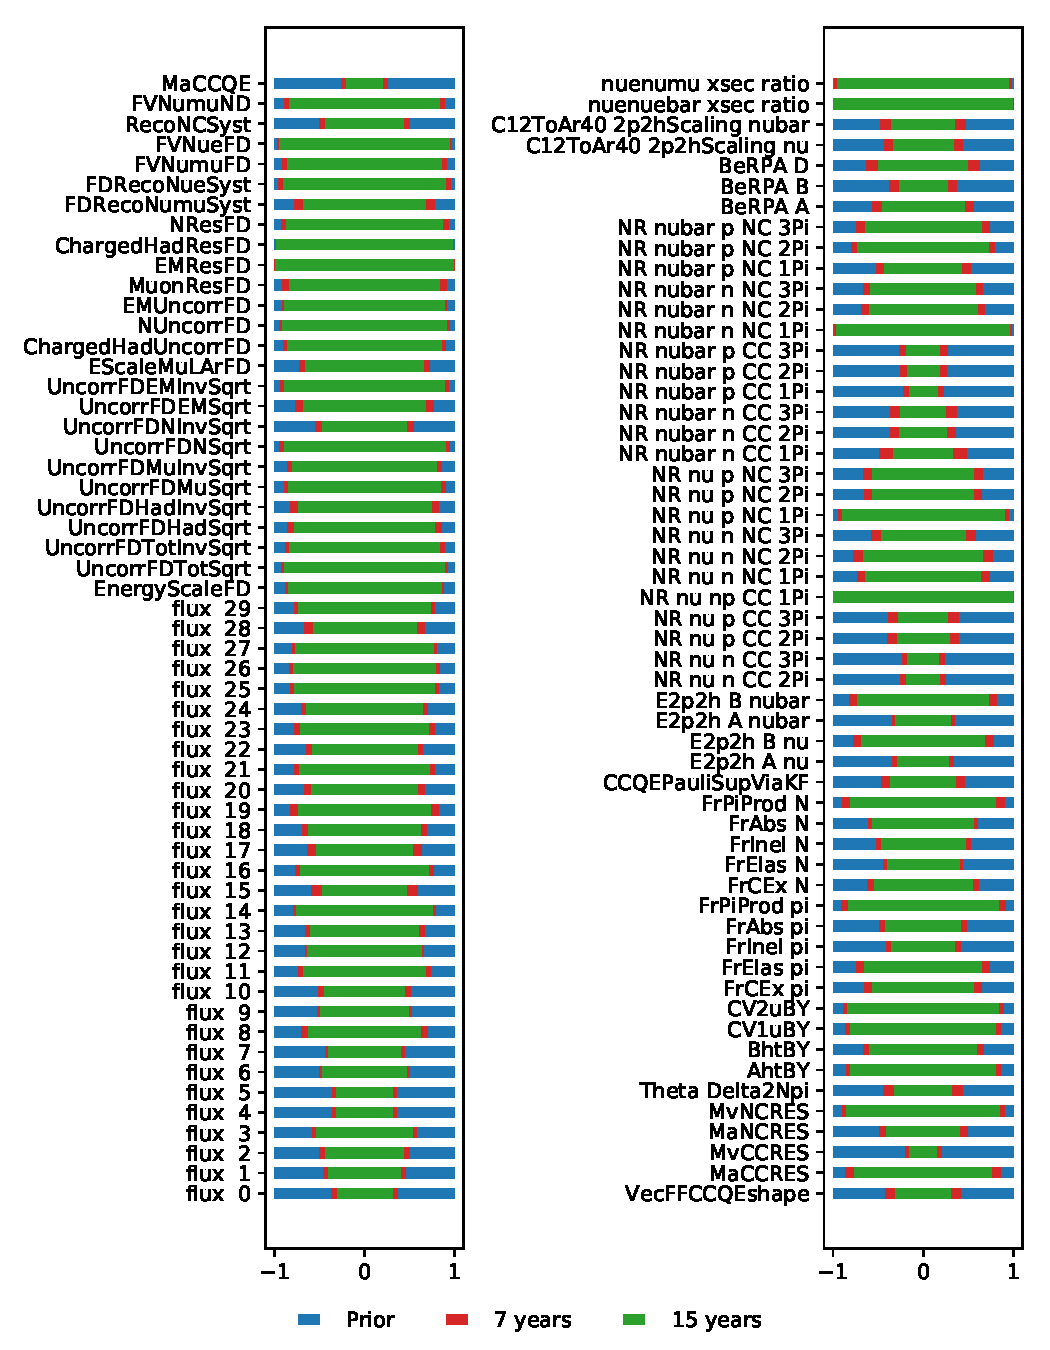
\includegraphics[width=0.8\textwidth]{nuisancePostFits_NDFD_7vs15_th13_v4_1.pdf}
\end{dunefigure}

%\subsubsection{Largest Systematic Uncertainties}

%The fits for this section are currently in progress.

%\fixme{Analysis in progress}

\subsection{Impact of the Near Detector}
\label{sec:ndimpact}

The oscillation sensitivity analysis presented in the previous section is intended to demonstrate the full potential of \dword{dune}, with constraints from the full suite of near detectors described in \introchnd, including the \dword{lar} \dword{tpc}, \dword{mpd}, 
% JU 1/24
%\dword{3dst}, 
\dword{sand}, 
% end JU 1/24
and off-axis measurements. In addition to the \numu and \anumu \dword{cc} spectra used explicitly in this analysis, the \dword{lar} \dword{tpc} is also expected to measure numerous exclusive final-state \dword{cc} channels, including 1$\pi^{\pm}$, 1$\pi^0$, and multi-pion production. Measurements will be made as a function of other kinematic quantities in addition to reconstructed $E_{\nu}$ and $y$, such as four-momentum transfer to the nucleus, lepton angle, or final-state meson kinematics. The \dword{lar} \dword{tpc} will also measure the sum of \nue and \anue \dword{cc} scattering, and \dword{nc} events. Direct flux measurements will be possible with neutrino-electron elastic scattering, and the low-$\nu$ technique.

In addition to the many on-axis \dword{lar} samples, a complementary set of neutrino-argon measurements is expected from the \dword{hpg} \dword{tpc}. This detector will be sensitive to charged tracks at kinetic energies of just a few MeV, enabling the study of nuclear effects in unprecedented detail. It will also sign-select all charged particles, with nearly perfect pion-proton separation from dE/dx out to over 1 GeV/c momentum, so that high-purity measurements of CC1$\pi^{+}$ and CC1$\pi^{-}$ are possible. It may be possible to directly measure neutron energy spectra from time of flight using the \dword{hpg} \dword{tpc} coupled to a high-performance \dword{ecal}. 
%
% JU 1/24
%The 3DST-S 
The \dword{sand} on-axis beam monitor
%
will measure neutrino-carbon scattering and neutron production while ensuring excellent beam stability.

The \dword{lar} and \dword{mpd} will also move off-axis to measure neutrino-argon interactions in many different fluxes. This will provide a direct constraint on the relationship between neutrino energy and visible energy in \dword{lar}. By taking linear combinations of spectra at many off-axis positions, it is possible to reproduce the expected \dword{fd} energy spectrum for a given set of oscillation parameters and directly measure visible energy.

All of these capabilities of the \dword{nd} benefit the \dword{dune} physics program. However, due to the timing of the \dword{nd} process, design details of the \dword{nd} are not available at the time of preparing this document, and it is not practical to include all of these samples and demonstrate their impact on oscillation sensitivity directly. Instead, we assume a model that implicitly includes these constraints, with further direct demonstration planned for the \dword{nd} \dword{tdr}.

The neutrino interaction model uncertainties shown in Section~\ref{sec:nu-osc-05} represent our current knowledge of neutrino interactions, motivated by measurements wherever possible. The \dword{dune} \dword{nd} is able to constrain these uncertain parameters, as demonstrated in the previous section. However, due to the complexity of modeling neutrino-argon interactions, and the dearth of neutrino-argon measurements in the energy range relevant for \dword{dune}, this is a necessary but insufficient condition for the \dword{nd} program. There are possible variations to the interaction model that cannot be readily estimated, simply because we have yet to observe the inadequacy of the model. While these ``unknown unknowns'' are impossible to predict, guarding against them is critically important to the success of the \dword{dune} physics program. For this reason, the \dword{nd} is designed under the assumption that it must not only constrain some finite list of model parameters, but also be sensitive to general modeling deficiencies.

The sensitivity analysis presented in the previous section assumes the success of the \dword{nd} program. Because of this assumption, in order to estimate the expected sensitivity without a \dword{nd}, it is not sufficient to simply remove the on-axis \dword{lar} \dword{nd} sample that is explicitly included in the analysis. We must also account for other potential biases from the interaction model, the ``unknown unknowns.'' In this section, we consider two simple examples of bias, and evaluate the potential impact on oscillation parameter measurements in a scenario where the \dword{nd} capacity is reduced. In Section~\ref{sec:FDonlyNuWro}, we consider the case where there is no near detector, and show a ``mock data'' sample that results in a high-quality \dword{fd}-only fit with a significant bias in the measured value of $\delta_{CP}$. This bias would be undetectable with a FD-only fit, but easily detected at the \dword{nd}. In Section~\ref{sec:missingProtonMD}, we consider an alternative mock data set that gives a high-quality fit to the \dword{fd} as well as the on-axis \dword{nd} spectra, but has significant biases that are easily detected with off-axis \dword{nd} data. These bias tests are not meant as exact estimates of the reduction in sensitivity that would be expected without a \dword{nd} or with only on-axis \dword{nd}, but they do serve as examples of the kind of bias that is possible. By estimating an additional uncertainty on oscillation parameters to cover the observed bias, it is possible to produce a sensitivity estimate; however, as it is based on one single possible bias, {\em it should be considered a lower bound on the potential reduction in sensitivity.}

\subsubsection{Bias study: \dword{fd}-only fit to NuWro}
\label{sec:FDonlyNuWro}

%An alternative Monte Carlo sample is produced by reweighting the \dword{genie} simulated events to \dword{nuwro} using a sophisticated multivariate framework that reproduces \dword{nuwro}-generated spectra in 18 kinematic quantities. 

An alternative Monte Carlo sample is produced by reweighting the \dword{genie} simulated events to \dword{nuwro}. The objective of the reweighting is to reproduce the \dword{nuwro} event spectra as a function of reconstructed neutrino energy, but without re-running the reconstruction. Simple reweighting schemes typically determine weights by taking the ratio between two generators in some limited kinematic space of true quantities. A common shortcoming of such techniques is that the reconstructed energy depends on many true quantities, and perhaps in a complicated way. Defining weights in a limited space effectively projects away any differences in other variables. To overcome this limitation, 18 true quantities that impact the reconstructed neutrino energy are identified: neutrino energy, lepton energy, lepton angle, $Q^{2}$, $W$, $x$, $y$, as well as the number and total kinetic energy carried by protons, neutrons, $\pi^{+}$, $\pi^{-}$, $\pi^{0}$, and the number of electromagnetic particles. A \dword{bdt} is trained on vectors of these 18 quantities in \dword{genie} and \dword{nuwro}. The \dword{bdt} minimizes a logistic loss function between \dword{genie} and \dword{nuwro} in the 18-dimensional space, producing a set of weights. When these weights are applied to \dword{genie} events, the resulting event spectra match the \dword{nuwro} spectra in all 18 quantities.

The resulting selected samples of \dword{fd} \numu and \nue \dword{cc} events in \dword{fhc} and \dword{rhc} beam modes are fit using the nominal \dword{genie}-based model and its uncertainties as described in Sections~\ref{sec:nu-osc-05} and \ref{sec:physics-lbnosc-syst}. The fit quality in the \dword{fd}-only scenario is high, with $\chi^{2}$ per degree of freedom smaller than unity for all oscillation parameters. Systematic nuisance parameters are pulled from their best fit values by more than $\sim$0.6$\sigma$. 

The best-fit value of $\delta_{CP}$ is determined for the full range of possible true $\delta_{CP}$ values between $-\pi$ and $+\pi$. The difference between the best-fit and true values of $\delta_{CP}$ is found to be less than 14 degrees for 68\% of the true values. To estimate the impact of such a bias on CP-violation sensitivity, an uncertainty equal to 14 degrees is added to the $\delta_{CP}$ resolution in quadrature. For a 10-year staged \dword{dune} \dword{fd} exposure, the resulting resolution is shown in the left panel of Figure~\ref{fig:nuwro_bias} compared to the nominal sensitivity with the \dword{nd} included. In the \dword{nd}+\dword{fd} (nominal) fit the bias is excluded, because in the \dword{nd} the bias is easily detected and not attributable to oscillations. To estimate the sensitivity to nonzero CP violation as shown in the right panel of Figure~\ref{fig:nuwro_bias}, the nominal \dword{fd}-only curve is reduced by the fractional increase in the $\delta_{CP}$ resolution at each point. The latter step is necessary because the uncertainty on $\delta_{CP}$ is not Gaussian.

\begin{dunefigure}[Oscillation sensitivities including example FD-only bias]{fig:nuwro_bias}
{The CP violation sensitivity for a \dword{fd}-only scenario with an additional uncertainty added to cover the observed bias from one example variation. The $\delta_{CP}$ resolution (left) and CP violation sensitivity (right) are compared to the results from the nominal \dword{nd}+\dword{fd} analysis.}
  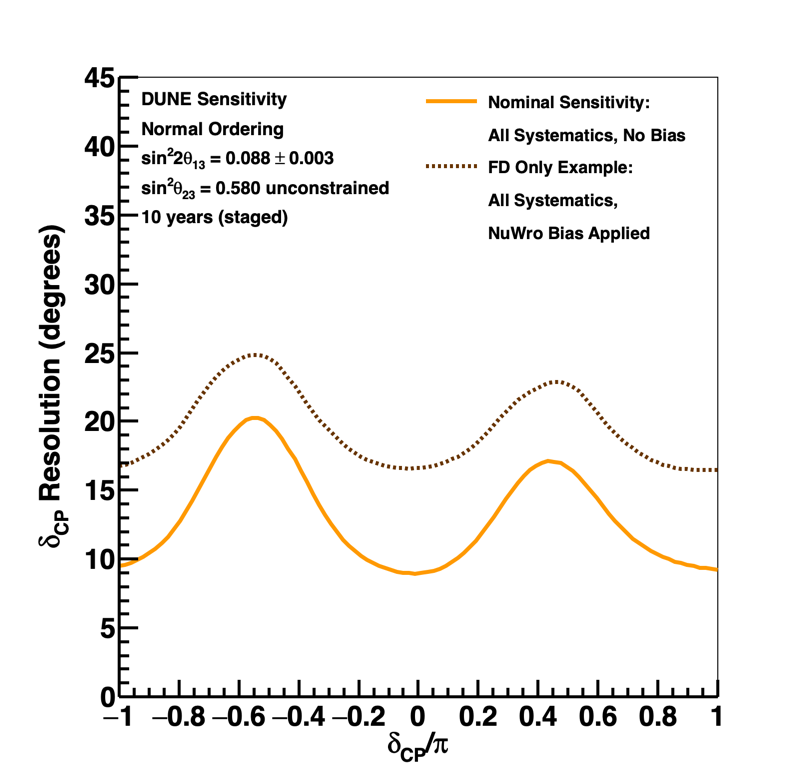
\includegraphics[width=0.48\textwidth]{dcpres_nuwrobias_2019_v4.png}
  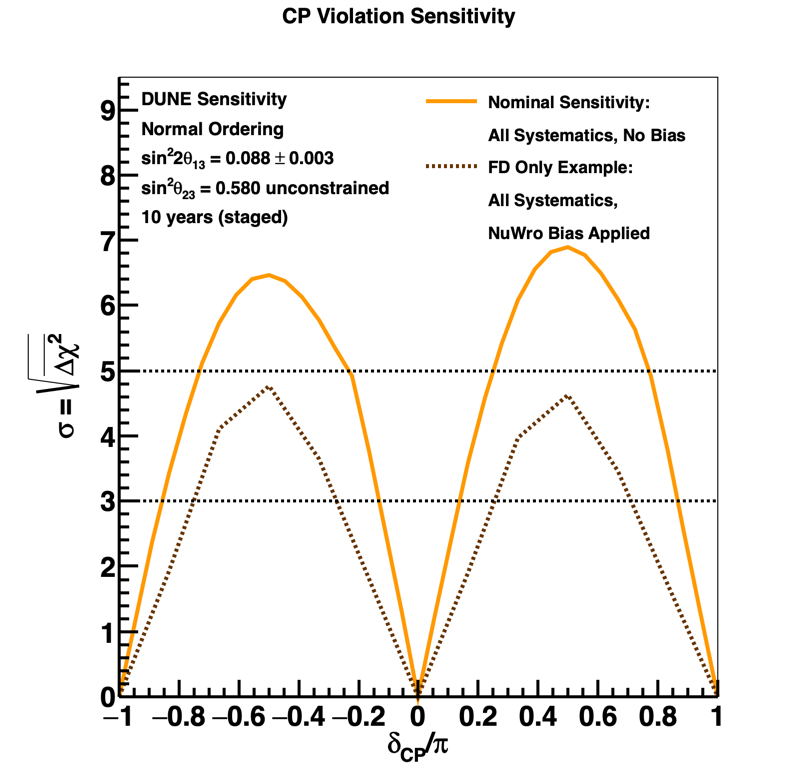
\includegraphics[width=0.48\textwidth]{cpv_nuwrobias_2019_v4.png}
\end{dunefigure}

As seen in Figure~\ref{fig:nuwro_bias}, the reduction in experimental sensitivity that would result from treating this example bias as a systematic uncertainty, which would be required in the absence of near detector data, is dramatic. Many other reasonable variations of the neutrino interaction model are allowed by world data and would also have to be considered as potential sources of uncertainty without near detector data to observe and resolve model incompatibility. 

\subsubsection{Bias study: shifted visible energy}
\label{sec:missingProtonMD}

As another example, we consider a possible deficiency of the \dword{genie} model, specifically the case where the energy of final-state protons is reduced by 20\%, with the energy going to neutrons instead. As neutrons are generally not observed, this will modify the relationship between neutrino energy and visible energy at the \dword{nd} and \dword{fd}. At the same time, the cross section model is altered so that the distribution of proton kinetic energy is unchanged. This alternate model is perfectly consistent with all available data; there is no reason to prefer our nominal \dword{genie} model to this one.

By construction, this alternate model will not affect the fit at the on-axis near detector, as the cross section shift exactly cancels the loss in hadronic visible energy due to changing protons for neutrons. Nuisance parameters that affect the near detector spectra, namely flux and cross section uncertainties, are not pulled and remain at their nominal values with the same post-fit uncertainties observed in the Asimov sensitivity. At the far detector, however, the different neutrino energy spectrum leads to an observed shift in reconstructed energy with respect to the nominal prediction, visible in Figure~\ref{fig:missingProton_spectra}.

\begin{dunefigure}[Shifted proton energy FD spectra]{fig:missingProton_spectra}
{Predicted distributions of reconstructed neutrino energy for selected \numu (top) and \nue (bottom) events, in \dword{fhc} (left) and \dword{rhc} (right) beam modes in 7 years. The black curve shows the nominal \dword{genie} prediction, while the red points are the mock data, where 20\% of proton energy is shifted to neutrons. The blue curve is the post-fit result, where systematic and oscillation parameters are shifted to match the mock data. The \dword{nd} spectra match the pre-fit prediction by construction and are not shown.}
  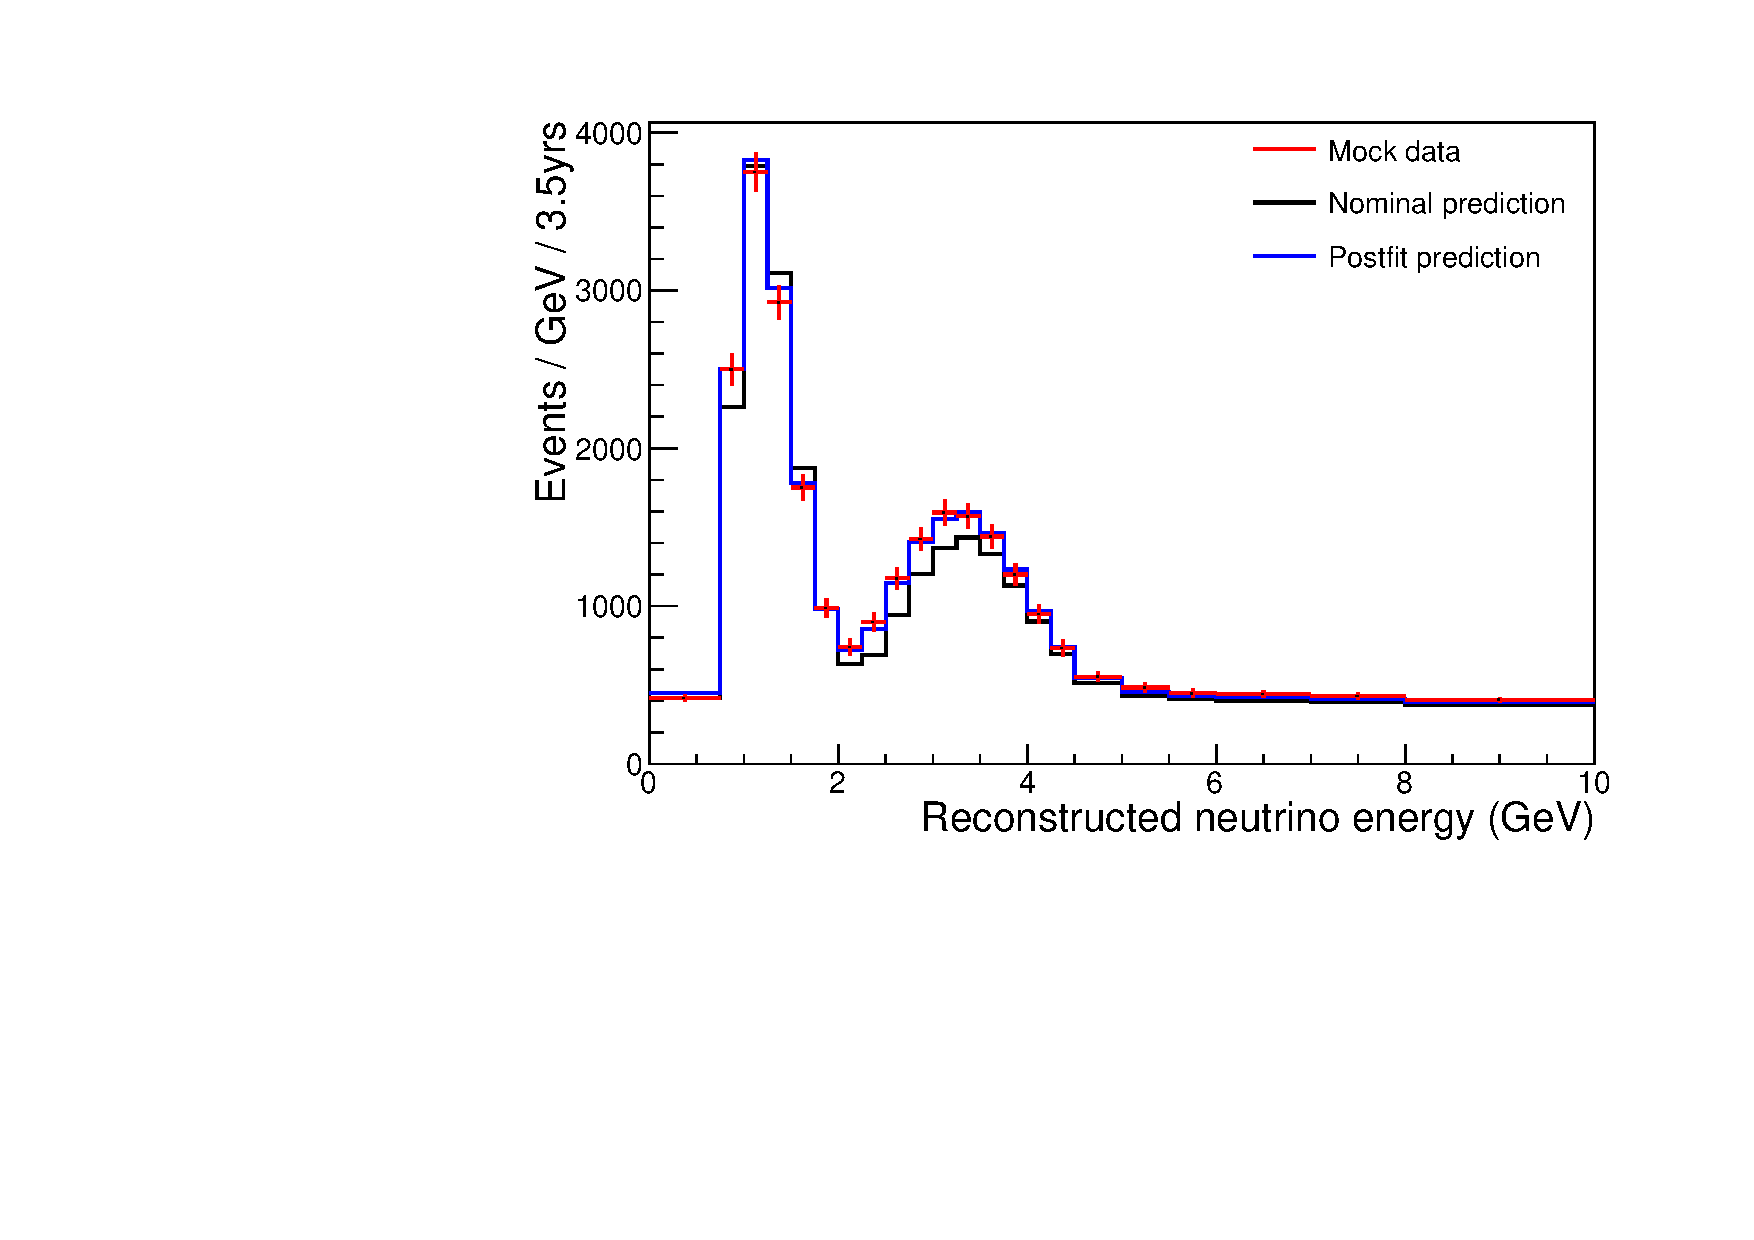
\includegraphics[width=0.45\textwidth]{missingProtonEnergyNDconstraint_NUMU_FHC_TDR.pdf}
  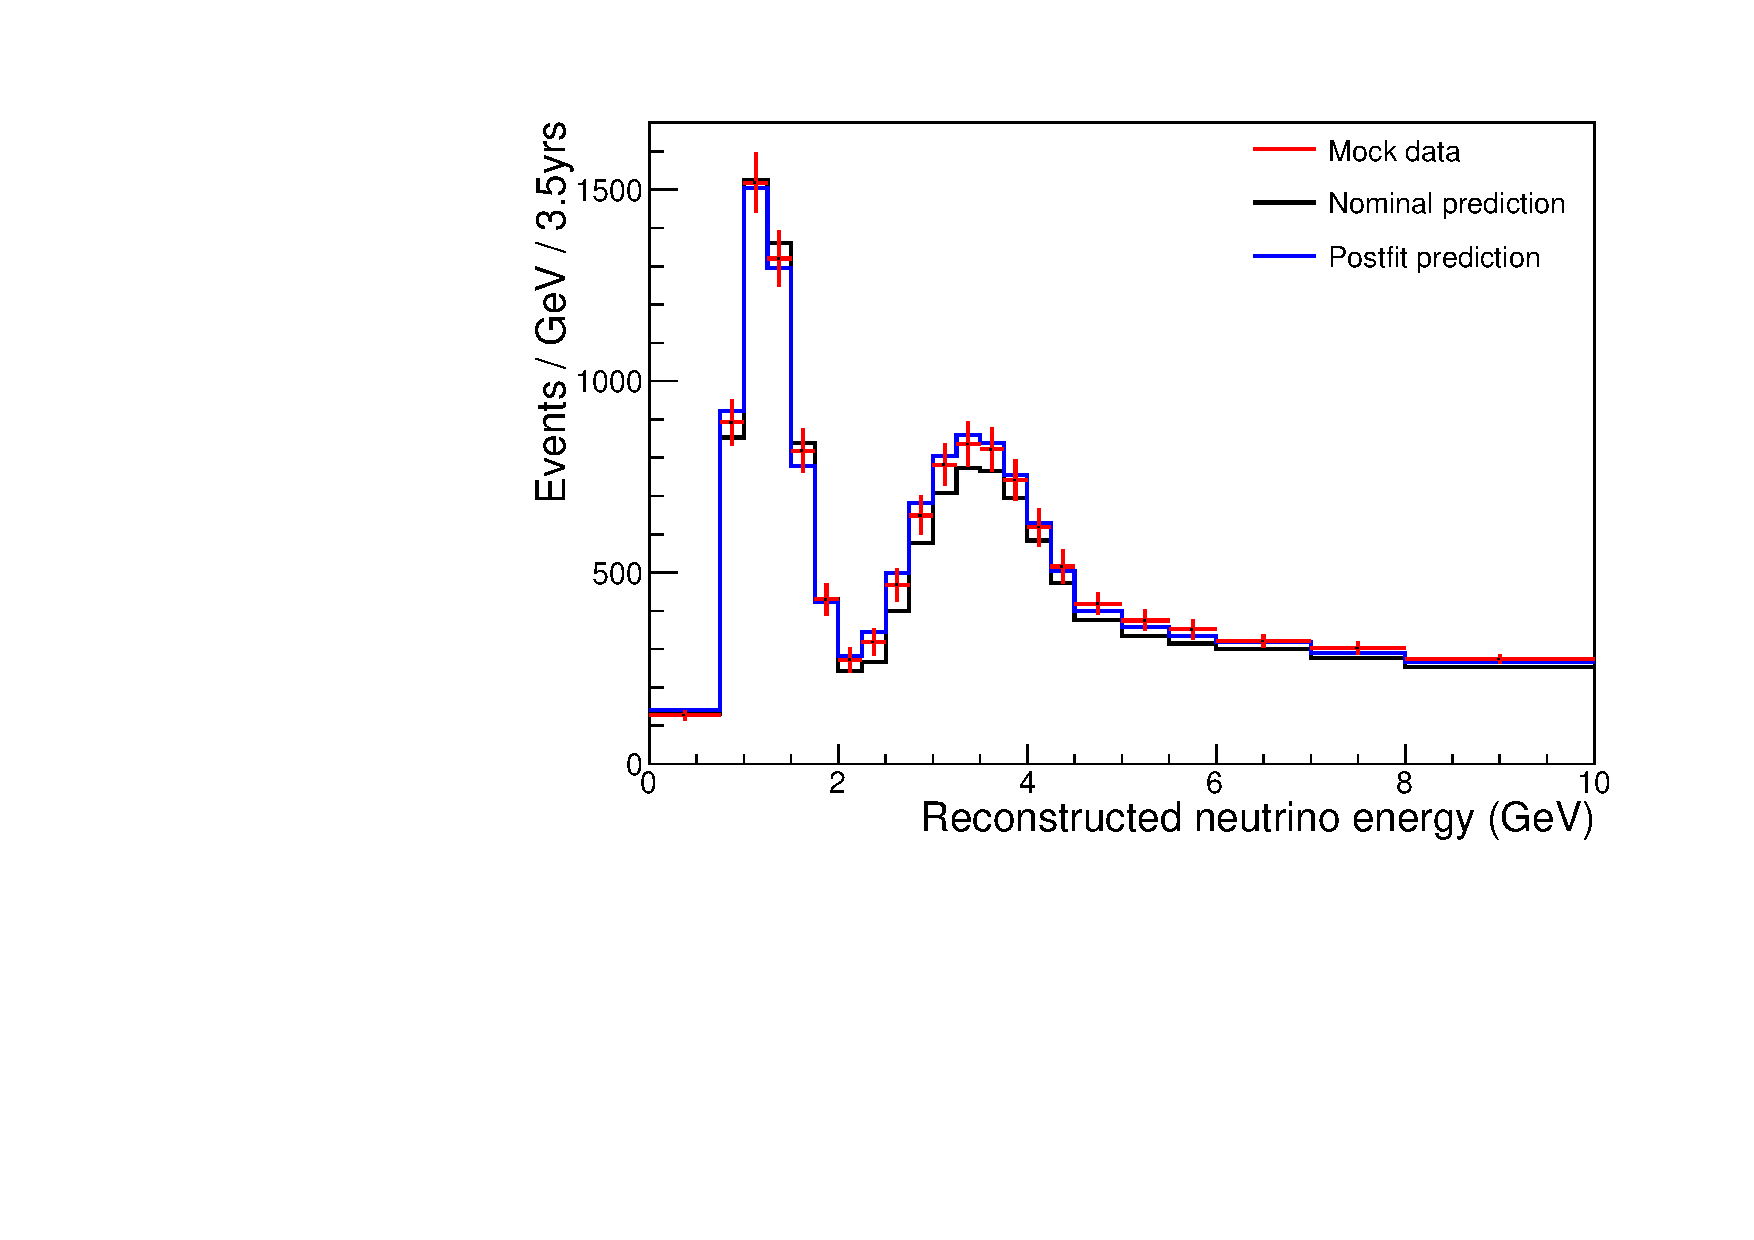
\includegraphics[width=0.45\textwidth]{missingProtonEnergyNDconstraint_NUMU_RHC_TDR.pdf}
  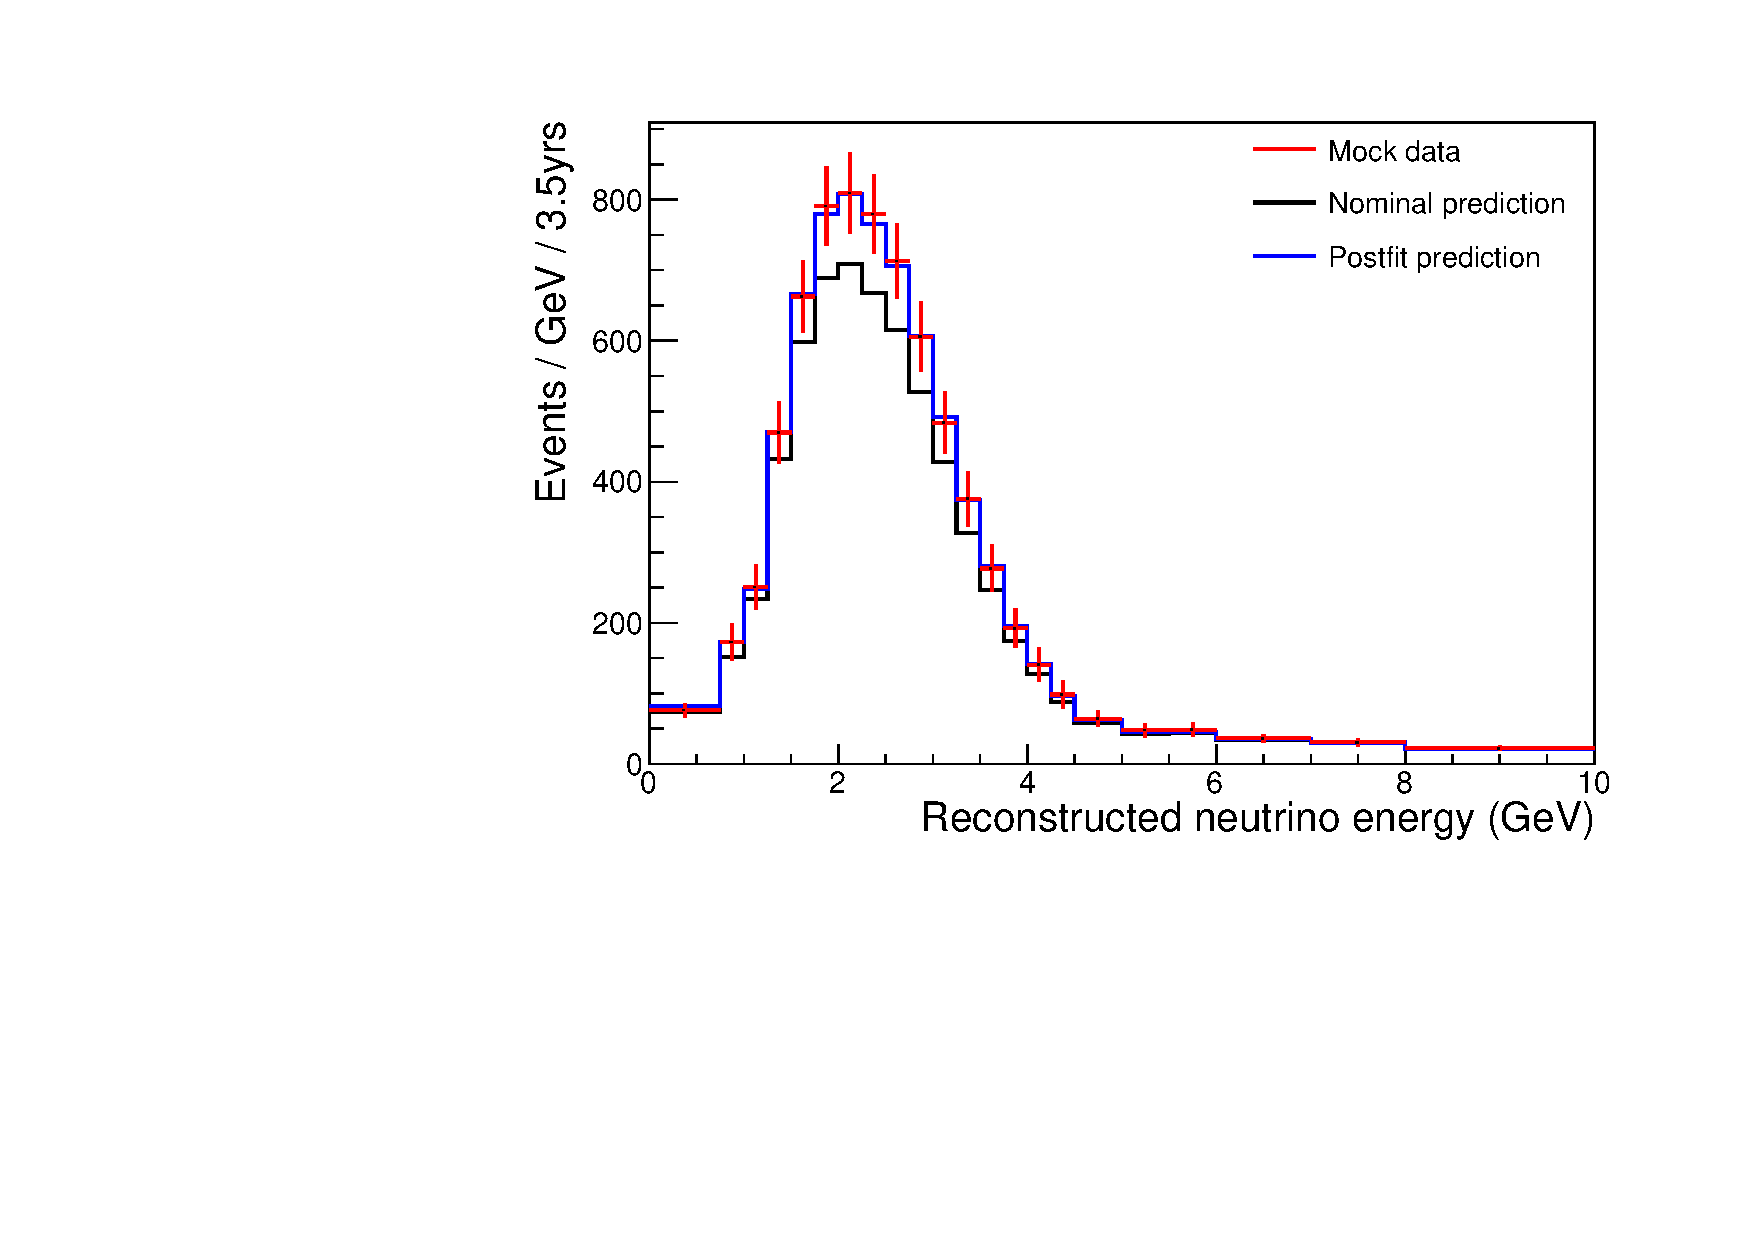
\includegraphics[width=0.45\textwidth]{missingProtonEnergyNDconstraint_NUE_FHC_TDR.pdf}
  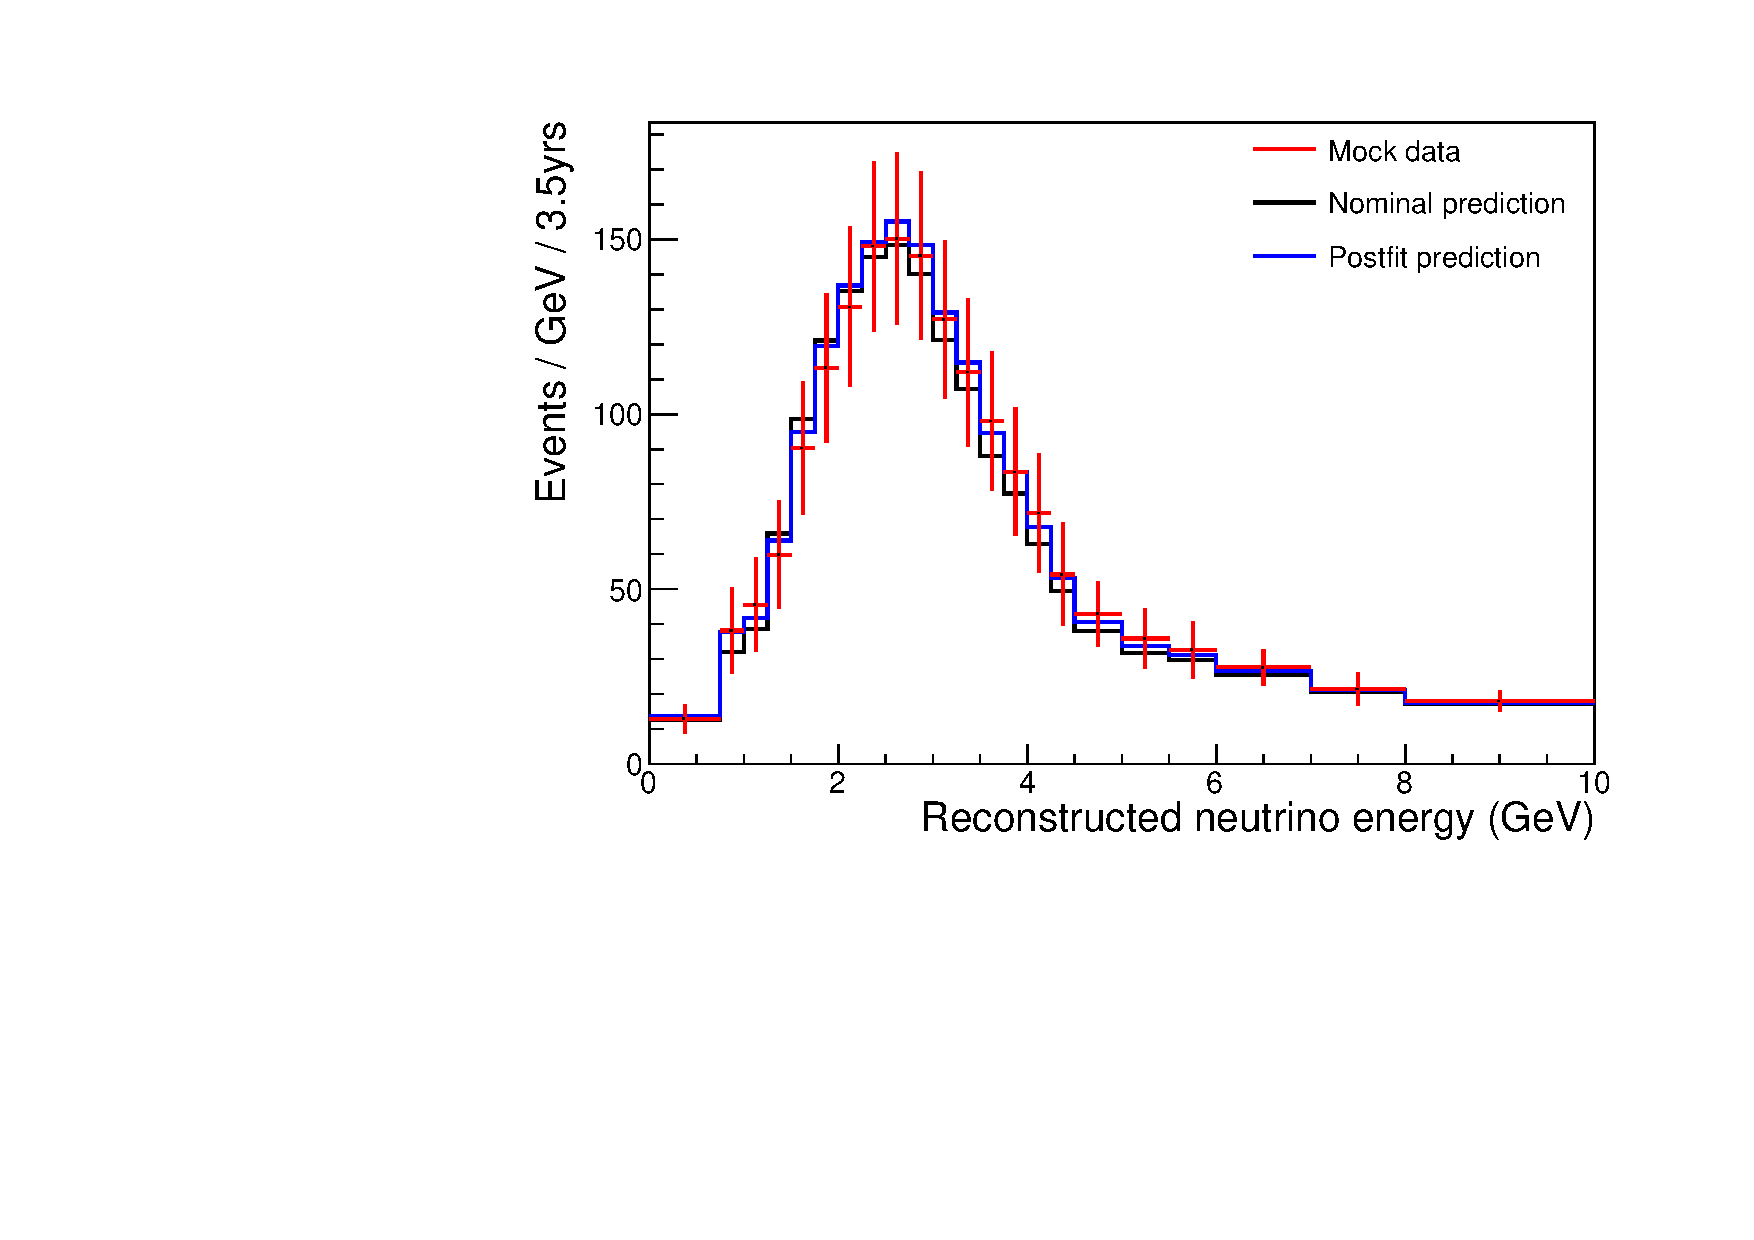
\includegraphics[width=0.45\textwidth]{missingProtonEnergyNDconstraint_NUE_RHC_TDR.pdf}
\end{dunefigure}

Measured oscillation parameters returned by this fit are biased with respect to their true values. In particular, the best-fit values of \dm{32} and sin$^{2}\theta_{23}$ are significantly incorrect, as shown in Figure~\ref{fig:missingProton_dm2th23}. Other parameters, including $\delta_{CP}$, happen not to be pulled significantly from their true values by this particular model variation.

\begin{dunefigure}[\dm{32}-sin$^{2}\theta_{23}$ contour for shifted proton energy]{fig:missingProton_dm2th23}
{Results of a fit to mock data where 20\% of proton energy is shifted to neutrons. The true values of \dm{32} and sin$^{2}\theta_{23}$ are given by the star, while the allowed 90\% C.L. regions are drawn around the best-fit point, for 7, 10, and 15 years of exposure. The solid region shows the result for a fit using the mock data, while the dashed curve shows the result for a fit using nominal simulation, for comparison.}
  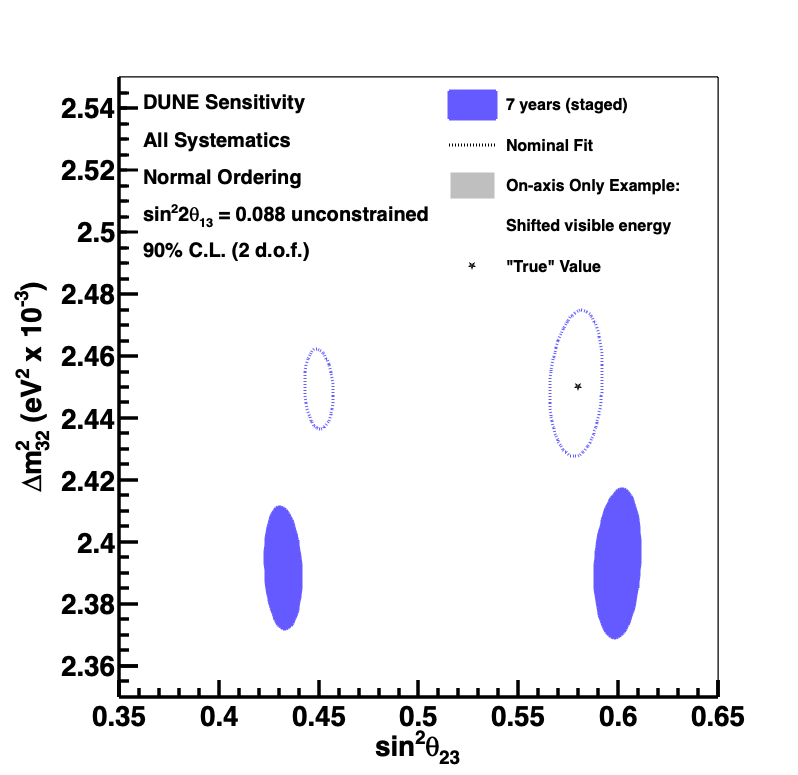
\includegraphics[width=0.5\textwidth]{bubbles_enerbybias.png}
\end{dunefigure}

While the nominal model gives a good fit to the mock data in the on-axis \dword{nd}, reconstructed spectra from off-axis \dword{nd} data give a poor fit. This occurs because the cancellation between the cross section shift and the final-state proton-to-neutron ratio is dependent on the true neutrino energy spectrum. Off-axis data access different neutrino energy spectra, where the relationship is broken. By combining data at many off-axis positions, it is possible to produce a data-driven prediction of the expected \dword{fd} flux for a given set of oscillation parameters, and directly compare this to the observation. Such a technique is not possible with solely on-axis \dword{nd} data. This example demonstrates the importance of a capable \dword{nd}, including the capability for off-axis measurements, to constrain not only the uncertain parameters of the interaction model, but also the physics in the model itself.




